% ============================================================
% Fighting in the Shadow of Intervention: A Learned-Proxy Analysis
% ============================================================

\documentclass[12pt]{article}


% ---- Fonts ----
%\usepackage[T1]{fontenc}
%\usepackage{libertine}
%\usepackage[libertine]{newtxmath}
\usepackage[scaled=0.85]{inconsolata}

% ---- Math ----
\usepackage{amsmath}
\let\Bbbk\relax  % resolve conflict between amssymb and newtxmath
\usepackage{amssymb}

% ---- Graphics and tables ----
\usepackage{graphicx}
\graphicspath{{figures/}}
\usepackage{booktabs}
\usepackage{multirow}
\usepackage{tabularx}

% ---- Citations (Chicago author-date) ----
\usepackage{natbib}
\bibliographystyle{chicago}

% ---- Cross-references ----
\usepackage[colorlinks=true, citecolor=blue, linkcolor=red, urlcolor=blue]{hyperref}

% ---- Misc ----
\usepackage{enumitem}

% ============================================================

\title{Fighting in the Shadow of Intervention:\\A Learned-Proxy Analysis}
\author{Robert J. Carroll}
\date{\today}

\begin{document}

% ---- Title page ----
\maketitle
\thispagestyle{empty}

\begin{abstract}

Theory predicts that anticipated third-party intervention shapes the
calculus of rebellion, yet no measure of expected intervention covers
the full population of potential interveners.  I construct one using a
two-stage learned-proxy design: a machine-learning ensemble predicts
the probability and direction of intervention for each directed
dyad-year; predictions are aggregated to a country-year shadow
disciplined by a Nash fixed-point condition.  Expected
government-biased intervention deters onset while expected
opposition-biased intervention encourages it.  The two shadow
variables are jointly significant ($p < 0.001$) despite wide
individual confidence intervals driven by inter-shadow collinearity,
and the directional pattern is robust across specifications,
measurement draws, and a country fixed-effects estimator.  The shadow
subsumes two leading existing proxies and carries out-of-sample
predictive content.
\end{abstract}

\noindent\textbf{Keywords:} civil war, military intervention, machine learning, learned proxy, onset

\noindent\textbf{Word count:} 7,635

\vfill
\begin{center}
\rule{\textwidth}{0.5pt}
\end{center}

% ---- Acknowledgments ----
% This paper has benefitted from discussions with Jeff Arnold,
% Quintin Beazer, Inken von Borzyskowski, Mike Colaresi, Tyson Chatagnier, Kevin
% Clarke, Casey Crisman-Cox, Amanda Driscoll, Kevin Fahey, Mark Fey, Nisha Fazal,
% Hein Goemans, Phil Henrickson, Gary Hollibaugh, Brenton Kenkel, Hye-Sung Kim,
% Bethany Lacina, Jeff Marshall, Will Moore, Jonathan Olmsted, Kai Ou, Matt
% Pietryka, Amy Pond, Pat Regan, Chris Reenock, Curt Signorino, Brad Smith,
% Mark Souva, Randy Stone, Susanna Supalla, and Jaroslav Tir.  The usual
% caveat applies.

\clearpage
\setcounter{page}{1}

% ============================================================
% Introduction
% ============================================================

A growing body of theory predicts that \textit{anticipated} third-party
intervention shapes civil war onset
\citep{cetinyan2002,cunningham2016,dudley2024,gibilisco2022,kuperman2008,kyddstraus2013,lango2023,sambanis2020},
yet the quantity has never been measured systematically.  No existing measure
covers the full population of potential interveners, varies annually with
shifting alliances and foreign policy alignments, and treats intervention
direction---government-biased versus opposition-biased---as the primary
quantity of interest.  This paper constructs such a measure and uses it
to test the hypothesis that the shadow of intervention deters and
emboldens.

The construction is the core contribution.  A machine-learning ensemble
trained on the \citet{regan2000} dataset of military
interventions (1946--2014) predicts, for each directed dyad in a given
year, the probability and direction of intervention.  Dyad-level
predictions are aggregated across all potential interveners to produce a
country-year shadow, disciplined by a Nash fixed-point condition
requiring each state's predicted probability to be self-consistent as an
input to the others' predictions.  The resulting measures are tested in
a standard country-year onset framework \citep{fearon2003}: expected
government-biased intervention enters negatively (deterrence), expected
opposition-biased intervention enters positively (emboldening), with the
directional pattern robust across specifications, measurement draws, and
a country fixed-effects estimator.

The closest existing approaches each sacrifice scope for
identification.  \citet{cunningham2016} uses the Lake
security hierarchy as a proxy for anticipated government-biased
intervention---a static, unidirectional measure restricted to the US
patron-client channel.  The present paper generalizes in three
directions: it covers all potential interveners, both sides of
intervention, and derives probabilities from a calibrated classifier
rather than structural position.
\citet{gibilisco2022} derive equilibrium intervention
expectations from a structural game among the P5, gaining clean
identification at the cost of restricting the player set to a size that
keeps joint-game estimation tractable.  In the Regan data, P5 states
account for fewer than half of all military interventions; the remaining
53 intervening states---neighbors, coethnics, regional rivals, Cold War
proxies---represent the majority of actual deployments and are driven by
logics qualitatively different from the global-order interests that
animate P5 behavior.  \citet{lango2023} develops a
formal model in which the threat of rebel-sided intervention can
simultaneously deter onset---by compelling governments to concede---and
encourage it---by raising rebels' expected return from fighting; the
utility parameters in the present framework can represent these
nonmonotone effects.

This paper takes a learned-proxy approach: a flexible first-stage model
constructs the latent quantity, and a parametric second-stage model tests
the theory.  This two-stage design is an increasingly common way to
bring machine learning into social science inference
\citep{knoxlucascho2022}, and arguably the least controversial
\citep{moruccispirling2024}: the ensemble does the measurement work it is
suited for, while the onset regression retains the interpretability that
causal claims require.  The design nests the structural functional
form---the unpenalized multinomial logit in the ensemble library directly
corresponds to the softmax best-response function of
\citet{gibilisco2022}---so whether that parametric
assumption fits the data is answered empirically rather than imposed by
construction.  (It earns less than one percent of the ensemble weight;
the data strongly prefer nonparametric alternatives.)

The learned-proxy approach has well-documented pitfalls.
\citet{knoxlucascho2022} catalog these systematically:
measurement-stage uncertainty is routinely ignored, proxy quality is
asserted rather than tested, and the disconnect between prediction and
inference is papered over.  This paper follows their recommendations
closely: Stage~1 performance is validated out-of-fold across 25
imputation draws; measurement uncertainty is propagated into Stage~2 via
a two-stage pairs cluster bootstrap that averages across all 25 draws;
calibration is verified by reliability diagrams; and a labeled-only
robustness check confirms that the onset estimates are not driven by
out-of-sample extrapolation.  The honest accounting of generated-regressor
uncertainty is itself a result: the corrected standard errors are roughly
2.9--3.5 times larger than naive MLE output, with a variance decomposition
showing that approximately 88--92\% of the total coefficient variance originates
in the measurement stage and only 8--12\% from primary-analysis sampling.  The
measurement model, not the regression, is the binding source of
uncertainty---precisely the situation \citet{knoxlucascho2022} warn about.
The two shadow variables are correlated at $r = 0.94$, which inflates
individual confidence intervals, but tested jointly they reject the
baseline at $p < 0.001$; the directional pattern holds across all 25
measurement draws, ten specifications, and country fixed effects.
The shadow subsumes both the Lake security hierarchy
\citep{cunningham2016} and the \citet{gibilisco2022} structural P5
estimates: neither adds explanatory power once the shadow variables are
included.

The paper proceeds as follows.  Section~\ref{sec:motivation} develops the theoretical
framework linking intervention expectations to the onset decision.
Section~\ref{sec:constructing} describes the construction and validation of the
shadow measure.  Section~\ref{sec:decision} presents the onset analysis, including
measurement-corrected inference and heterogeneous-utility extensions.

% ============================================================
% Intervention and the Onset Decision
% ============================================================

\section{Intervention and the Onset Decision}
\label{sec:motivation}

What does it mean, formally, for an opposition group to act in the shadow
of intervention?  This section develops a model of the onset decision that
derives the functional form that intervention expectations must take to be
both theoretically coherent and empirically tractable.

\subsection{The Model}

\begin{figure}[t]
  \centering
  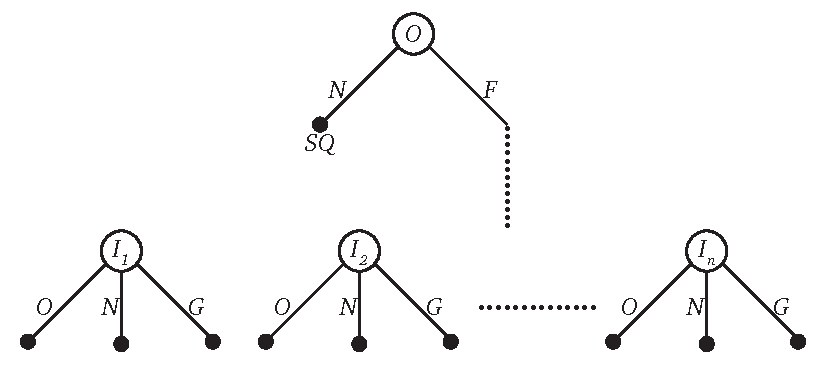
\includegraphics[width=0.85\textwidth]{ntree.pdf}
  \caption{Motivating formal model.}
  \label{fig:ntree}
\end{figure}

The decision problem is depicted in Figure~\ref{fig:ntree}.  An opposition group $O$
chooses whether to Fight ($s_O = F$) or Not fight ($s_O = N$).  Should it
not fight, the game ends at the status quo $SQ$.  If it fights, $n$
potential interveners simultaneously choose actions $s_i \in \{O, N, G\}$---
opposition-biased, non-intervention, or government-biased---and the
combined profile $s \in S = \{O, N, G\}^n$ determines the international
environment the opposition faces.

Each potential intervener $i$ has a utility function $u_i : S \rightarrow \mathbb{R}$
over profiles.  Under expected utility, let $\sigma_i$ be a probability
measure over $\{O, N, G\}$, and let
$U_i(\sigma) = \sum_{s' \in S} u_i(s') \prod_j \sigma_j(s'_j)$.
A Nash equilibrium $\sigma^*$ of the intervention subgame satisfies
$U_i(\sigma_i^*, \sigma_{-i}^*) \geq U_i(\sigma'_i, \sigma_{-i}^*)$
for every $\sigma'_i$ and every $i$.  The equilibrium profile feeds back
to the opposition, whose expected utility of fighting is
$U_O(F; \sigma^*) = \sum_{s' \in S} u_O(s') \prod_i \sigma_i^*(s'_i)$.
A subgame perfect equilibrium requires that $\sigma^*$ be a Nash equilibrium
of the intervention subgame and that

\begin{equation*}
u_O(SQ) \geq U_O(F; \sigma^*) \iff s_O^* = N.
\end{equation*}

The opposition fights if and only if the expected return to fighting, given
equilibrium intervention, exceeds the status quo.  The international
environment enters the calculus entirely through $\sigma^*$: the anticipated
behavior of outside powers can make the difference between peace and war
before a single shot is fired.  This is the shadow of intervention
\citep{cetinyan2002}.\footnote{%
  Whether $\sigma^*$ approximates the expectations that rebels actually form
  is not merely assumed.  Under rational expectations, agents exploit
  available information at least as well as the researcher's model
  \citep{muth1961}.  The Stage~1 classifier described in Section~\ref{sec:constructing}
  recovers a substantial share of the predictive content in realized
  intervention outcomes using only publicly observable state
  characteristics; rebels who can also draw on private intelligence,
  direct patron relationships, and local knowledge face a forecasting
  problem that is easier, not harder, than the one the classifier solves.}

\subsection{From Equilibrium to Empirics}

The equilibrium condition is theoretically exact but empirically intractable
as stated.  With up to 193 potential interveners each choosing among three
options, the expectation over $U_O$ runs over $3^{192}$ profiles---larger
than the number of elementary particles in the observable universe.  Two
assumptions reduce the problem to a tractable form without discarding its
theoretical content.

\textbf{Assumption 1 (Separability).}  The opposition's payoff from any profile
is additive across interveners:
$u_O(s') = \sum_i u_O^i(s'_i)$, where $u_O^i : \{O, N, G\} \rightarrow \mathbb{R}$
measures the marginal contribution of intervener $i$'s action.

Separability captures a specific and substantively defensible theory of how
opposition groups aggregate international expectations: each outside power's
likely behavior enters the calculus independently, and the combined effect
is their sum.  A rebel coalition assessing its international environment in
1970s Angola had a view about what Cuba would likely do, a separate view
about South Africa, and a separate view about the United States; the
hypothesis is that these entered additively.  The assumption rules out
complementarities---the value of Soviet logistics may depend on whether
Cuban troops are also present---but coordinated multilateral operations
constitute a small minority of actual interventions.\footnote{%
  \citet{aydinregan2011} find that the \textit{alignment} among interveners matters for
  civil war duration: same-side interventions shorten wars only when the
  intervening states share similar preferences.  This is evidence of
  complementarities in the conduct phase.  Separability here pertains to
  the onset calculus---the rebel's assessment of the intervention
  environment at the moment it decides whether to fight---not to the
  downstream interactions among interveners once fighting begins.  The
  spatial lags in the Stage~1 classifier (Section~\ref{sec:constructing}) capture
  interdependence among interveners' \textit{choices} without requiring that
  their \textit{effects} on the rebel enter non-additively.}

Separability also enables the extension to the full system of potential
interveners.  Because each state's contribution enters Equation~\eqref{eq:EU} additively,
computing the opposition's expected utility requires only the marginal
intervention probabilities $\sigma_i$---not the joint distribution over all
$n$ players' actions simultaneously.  Specifying and estimating the full
joint game---the approach of \citet{gibilisco2022} for the
five permanent Security Council members---becomes computationally
intractable beyond a small player set.  Separability sidesteps that
constraint while preserving the game's central implication: the equilibrium
strategies of outside powers must be mutually consistent.  That consistency
requirement is enforced directly via the Nash fixed-point iteration
described in Section~\ref{sec:constructing}.

\textbf{Assumption 2 (Non-intervention as reference).}  For all $i$,
$u_O^i(N) = 0$.  This normalization makes the intervention-free onset
model a limiting case: if no state intervenes, the expected utility of
fighting reduces to purely domestic considerations, and the standard
country-year onset model follows directly.

Under these two assumptions, the expected utility of fighting simplifies to

\begin{equation}
U_O(F; \sigma) = \sum_{i=1}^{n} \left[\sigma_i(O)\, u_O^i(O) + \sigma_i(G)\, u_O^i(G)\right].
\label{eq:EU}
\end{equation}

Equation~\eqref{eq:EU} is the primary theoretical object, and the two-stage empirical design
follows directly from its structure.  The equation contains two types of
unknowns: the intervention probabilities $\sigma_i(O)$ and $\sigma_i(G)$,
and the marginal utilities $u_O^i(O)$ and $u_O^i(G)$ that scale each.
Stage~1 (Section~\ref{sec:constructing}) estimates the probabilities for every directed
dyad using a machine-learning classifier trained on the Regan intervention
record.  Stage~2 (Section~\ref{sec:decision}) recovers the utility parameters from their
aggregate effect on civil war onset.  The theory does not merely motivate
the empirical strategy; it specifies exactly what each stage must estimate
and how the estimates connect.

The model assigns the strategic decision to the opposition, not because
governments are passive but because this is where the onset decision
sits---following the literature's longstanding focus on the conditions that
facilitate or inhibit insurgency \citep{fearon2003}.  Governmental behavior enters
implicitly through the opposition's status quo utility and the host-country
features in the Stage~1 classifier; endogenizing the government's response
would require a bargaining game that severs the tight deductive connection
between Equation~\eqref{eq:EU} and its empirical counterpart.

% ============================================================
% A Learned Proxy for the Shadow of Intervention
% ============================================================

\section{A Learned Proxy for the Shadow of Intervention}
\label{sec:constructing}

Operationalizing the shadow requires a measure of the expected intervention
environment at the moment a potential rebel group weighs the costs and benefits
of open conflict.  The construction proceeds in two stages: a directed-dyad
classifier estimates intervention probabilities for every potential
intervener, and a country-year aggregation sums them under a Nash
fixed-point condition ensuring self-consistency.

\subsection{Outcome Variable}

The Stage~1 training labels draw primarily from \citet{regan2000},
whose dataset records third-party military, economic, and diplomatic
interventions in civil conflicts from 1944 to 1999.  I extend Regan's coding
through 2014 by hand-coding unambiguous military interventions in post-1999 COW
onset country-years.  The coding threshold requires deployment of military
personnel---troops, combat advisors, or directed proxy forces attributable to a
specific state---on behalf of one side; arms transfers, economic aid, and
sanctuary alone are insufficient.  UN peacekeeping missions are excluded.  The
post-1999 extension adds 31 directed dyad-year records across 14 host countries,
yielding a combined intervention table of 455 records (1944--2014); the full
coding with source notes appears in Online Appendix~\ref{app:coding}.

The civil war universe is drawn from the Correlates of War Intra-State War
Dataset (v5.1) \citep{dixon2016}, restricting to wars fought for central control
(type~4) or local/secessionist issues (type~5).  The COW threshold
($\geq$1,000 battle deaths) is theoretically appropriate: the mechanism requires
rebels organized enough to form rational expectations and conflicts large
enough that outside military involvement is a realistic prospect.\footnote{%
  At lower thresholds---such as the UCDP/PRIO $\geq$25-death criterion---third-party
  military intervention becomes vanishingly rare, swamping any predictive signal.}
This yields 153 distinct onset country-years between 1946 and 1999 and 191
through 2014.  I restrict attention to \textit{military} interventions, coded as
\textit{government-biased}~(1) or \textit{opposition-biased}~(2); corrections and
deduplication are documented in Online Appendix~\ref{app:coding}.

For each directed dyad $(B \rightarrow A)$ active in a civil war onset year, the
training label is: 0 (no military intervention), 1 (government-biased), or 2
(opposition-biased).  Non-onset dyad-years are excluded from the training set.
This produces 254 intervention-coded onset observations---150 government-biased
and 104 opposition-biased---across 51 host countries and 58 unique intervening
states.  The five permanent Security Council members
account for 110 of these events (43~percent); the remaining
states---Cold War proxies, neighbors, regional patrons, and coethnics---account
for the majority (Table~\ref{tab:interveners}).

Training exclusively on onset country-years is not a convenience---it is
the only option.  Intervention in a civil war is undefined absent a civil war;
in non-onset years the outcome is not ``zero intervention'' but rather
unobserved.  The consequence is that the training sample is selected on
precisely the outcome that the Stage~2 analysis tries to explain: if the
shadow deters onset, then high-shadow country-years are systematically
underrepresented among onsets, and the classifier learns the
feature--intervention mapping from an endogenously filtered sample.  There
is no design that avoids this.  The defense rests on what the classifier
is asked to learn.  The training target is the conditional relationship
between \textit{dyad-level} features---alliance portfolios, capability ratios,
colonial ties, geographic proximity, regime similarity---and the direction
of military intervention, given that a war has started.  These bilateral
characteristics are plausible determinants of how state $B$ behaves toward
state $A$ in a conflict regardless of what brought that conflict about.
The fixed-point iteration then
handles the extrapolation: it asks what the equilibrium intervention
environment \textit{would} look like in any country-year, including those where
onset was never observed, without requiring that the training sample be
representative of the full population.

\begin{table}[t]
  \centering
  \begin{tabular}{@{}lrrr@{}} 
    \toprule
    State & Gov. & Opp. & Total \\
    \midrule
    United States\textsuperscript{\dag}   & 31 & 15 & 46 \\
    USSR / Russia\textsuperscript{\dag}   & 16 &  7 & 23 \\
    United Kingdom\textsuperscript{\dag}  &  9 &  8 & 17 \\
    France\textsuperscript{\dag}          & 11 &  6 & 17 \\
    Cuba                                  &  7 &  1 &  8 \\
    China\textsuperscript{\dag}           &  2 &  5 &  7 \\
    Libya                                 &  1 &  6 &  7 \\
    Iran                                  &  2 &  5 &  7 \\
    Somalia                               &  0 &  5 &  5 \\
    Syria                                 &  3 &  2 &  5 \\
    India                                 &  4 &  1 &  5 \\
    Uganda                                &  3 &  2 &  5 \\
    \bottomrule
  \end{tabular}
  \caption{Most frequent military interveners (1946--2014); states with
    fewer than five interventions omitted.
    \textsuperscript{\dag}~Permanent member of the UN Security Council (P5).
    Government-biased (Gov.)\ and opposition-biased (Opp.)\ interventions
    are coded from the Regan \texttt{target} variable and post-1999 extension.}
  \label{tab:interveners}
\end{table}

\subsection{Feature Set}

The classifier draws on 105 directed-dyad-year features organized
around four substantive dimensions (full list in Online Appendix~\ref{app:varlist}).
Many variables enter twice---once for the potential intervener and
once for the host---so that the classifier can learn asymmetric effects.
Missing data are multiply imputed using miceforest (five country-year
$\times$ five undirected-dyad imputations, yielding 25 complete datasets;
Online Appendix~\ref{app:imputation}).

\begin{itemize}
\item \textbf{State characteristics of both the potential intervener and the host.}
  Material capabilities (CINC scores and components, GDP, population) from COW
  v6 \citep{singer1987} and V-Dem v15 \citep{vdem2025}; regime type (Polity~II and lags,
  liberal democracy index, instability); power status (COW major power, P5
  membership); and host-side conflict history, ethnic fractionalization
  \citep{fearon2003}, ethnic exclusion \citep{cederman2010}, oil wealth, and terrain.

\item \textbf{Bilateral ties.}  Alliance commitments \citep{gibler2009}, bilateral trade,
  geographic proximity (log capital distance, contiguity \citealp{stinnett2002}),
  colonial history, territorial disputes \citep{huth2003}, expected dispute outcomes
  \citep{carroll2019}, and peace quality \citep{diehl2019}.

\item \textbf{Foreign policy alignment.}  UN General Assembly ideal points
  \citep{bailey2017} for each state and the absolute distance between them;
  shared IGO membership from COW Dyadic IGO v3 \citep{pevehouse2020}.

\item \textbf{Spatial context.}  Ten spatial lag variables constructed from a
  row-normalized polity-similarity weight matrix capture the weighted behavior
  of other potential interveners in the same host-year: the fraction
  coded government- or opposition-biased, US and Soviet intervention
  posture, and four superpower interaction terms \citep{gent2007,salehyan2007}
  (Online Appendix~\ref{app:spatial}).
\end{itemize}

Before training, the 115 features (95 dyadic covariates + 20 spatial lags) are
standardized and reduced via principal components analysis, retaining components
to 90\% of cumulative variance (59--61~components across all 25 imputation
datasets).

\subsection{Classifier Design}

The multinomial outcome (0 = no intervention, 1 = government-biased,
2 = opposition-biased) is modeled using a super-learner ensemble
\citep{vanderlaan2007}.

Nine component classifiers spanning three model families are trained
within a ten-fold cross-validation scheme: two tree ensembles (a random
forest \citealp{breiman2001} and two histogram-based gradient boosting
specifications at different learning rates), four logistic regression variants (ridge,
elastic-net, lasso, and unpenalized multinomial), and two multi-layer
perceptrons (shallow and deeper architectures).  The unpenalized
multinomial logistic regression---a softmax best-response function---directly
nests the functional-form assumption of structural game-theoretic models of
intervention \citep{gibilisco2022}; its stacking weight is determined by
out-of-fold predictive performance, so whether that assumption fits the data
is answered empirically rather than imposed by construction.  Each
classifier produces a vector of class probabilities for every
training observation.  The super learner combines these using
non-negative least squares (NNLS) weights chosen to minimize held-out
multinomial log-loss, so that the ensemble adaptively up-weights
component classifiers that predict well on out-of-fold observations.

All reported performance statistics are based on out-of-fold
predictions to guard against overfitting---following \citeauthor{wang2018}'s
(\citeyear{wang2018}) demonstration that
evaluation of class-imbalanced political-event models on training data
produces severely inflated performance estimates \citep{muchlinski2016}.
The primary performance metric is the proportional reduction in log-loss
relative to the class-frequency null model (PRL); the area under the ROC
curve (AUC) is also reported.

\paragraph{Spatial lags and Nash fixed-point iteration.}
The broader motivation for
the two-stage design is that intervention decisions are endogenous to the
conflict environment: interveners select into conflicts strategically, and
a single-equation model that treats realized intervention as a covariate in
an onset regression conflates the causal effect with the selection process
that generated it \citep{signorino2002,gent2008}.  Qualitative evidence confirms
the problem directly: rebel groups in Bosnia and Kosovo explicitly
conditioned their onset decisions on anticipated outside support, so
realized intervention is partly a consequence of expected intervention
rather than an independent cause \citep{kuperman2008}.  Using predicted
intervention expectations rather than realized intervention is the
appropriate correction.

The spatial context variables described in Appendix~\ref{app:spatial} depend on the
intervention choices of \textit{other} potential interveners---quantities that are
themselves to be predicted.  A documented pattern of countervailing
intervention makes these dependencies quantitatively important: when one
state intervenes on the government side, ideologically rival states face a
selective incentive to support the opposition, and vice versa \citep{salehyan2011,findleyteo2006}.
\citet{aydinregan2011} confirm that these
network effects are consequential: opposing interventions nearly double civil
war duration, while same-side interventions shorten wars only when the
intervening states share similar foreign policy preferences---evidence that
the strategic alignment among interveners, not merely their count, carries
the signal.  This creates a concrete measurement problem.
Without an explicit consistency requirement, spatial lags are computed
from \textit{observed} training-data intervention choices, which are not the
model's own outputs.  Applied out-of-sample---to country-years unlike
the training-period equilibrium---the predictions embed a deterministic
discrepancy between lag inputs and probability outputs whose sign and
magnitude depend on how far the out-of-sample world departs from
training-period behavior.  This is systematic error, not sampling noise,
and in a measure designed to capture counterfactual intervention
environments the bias could be large.

The fix is to require that the predictions be self-consistent inputs to
themselves:

\begin{equation}
\sigma^*(B, A, t) = \hat{M}(X(B, A, t, \sigma^*)) \quad \forall\, (B, A, t),
\label{eq:fp}
\end{equation}

\noindent where $\hat{M}$ is the trained super-learner classifier.  At $\sigma^*$,
the spatial lags are derived from the model's own equilibrium predictions,
not from historical observations.
The deterministic discrepancy disappears by construction.

This self-consistency condition is also the Nash equilibrium condition
for a natural class of games.  The primitive object is the best-response
correspondence, not the game itself: a game specifies a best-response
correspondence \textit{derivatively}, via utility maximization; $\hat{M}$ specifies
one \textit{directly}, from the data.  Nash equilibrium is a fixed point of
the best-response correspondence and does not require identifying the
payoff functions that generate it.  Games can be partitioned into
equivalence classes under the relation ``generates the same best-response
correspondence''; $\sigma^*$ is the Nash equilibrium of every game in the
class whose correspondence $\hat{M}$ estimates.\footnote{%
  The set of rationalizing payoff functions for any interior $\sigma^*$
  is non-empty---choose utilities that make each player indifferent among
  actions assigned positive probability.  What is identified is the
  correspondence; the payoffs that generate it are not.  A natural
  parametric fiber of these classes is the linear-utility family
  $u_i(a, \sigma_{-i}) = \alpha \cdot f_i(a) + \beta \cdot W_i(a, \sigma_{-i})$,
  where $f_i$ captures state-specific intervention incentives and $W_i$
  the spatial interaction term.  The best-response from this family is a
  softmax---the functional form of the multinomial logit component of
  the super-learner---so the parametric case is explicitly represented
  in the ensemble while the broader non-parametric mixture accommodates
  departures from it.  The iterative procedure that solves Equation~\eqref{eq:fp}
  is the nonparametric analogue of the nested pseudo-likelihood (NPL) algorithm
  of \citet{aguirregabiriamira2007}: the fitted
  super-learner replaces the parametric best-response function,
  and the fixed-point iteration updates beliefs (spatial lags) until
  self-consistency, as in A\&M's two-step PML.  In the parametric case,
  \citet{crismancox2021} show that this class of
  iterative estimators substantially outperforms direct maximum likelihood
  estimation of strategic games under equilibrium multiplicity.
  Uniqueness of the fixed point is not guaranteed in general, but
  convergence is rapid (two to three passes across all 25 imputation
  draws), consistent with a contractive mapping.}
If the training data reflect equilibrium play and the spatial lags are
sufficient statistics for the strategically relevant information in
$\sigma_{-i}$, then $\hat{M}$ is a non-parametric estimate of the true
best-response correspondence $\mathrm{BR}^*$ and $\sigma^*$ estimates its fixed
point, without specifying which game in the equivalence class is the
true data-generating process.  The statistical
and game-theoretic justifications therefore coincide: Equation~\eqref{eq:fp} corrects a
concrete measurement error and simultaneously identifies the equilibrium
of the underlying intervention game, whichever member of the equivalence
class that game happens to be.

Equation~\eqref{eq:fp} has no closed form but is solved by fixed-point iteration.
The iteration proceeds in two stages.  In the \textit{training stage}, the
classifier is first fit using observed spatial lags; out-of-fold predictions
then replace the observed intervention indicators to recompute spatial lags;
and the classifier is refit on the updated lags.  This loop repeats until
convergence, typically within two to three passes.  In the \textit{prediction
stage}, the trained classifier is held fixed and only the spatial lags are
updated: the model predicts for every directed dyad-year (onset and non-onset
alike), spatial lags are recomputed from those predictions, and the model
re-predicts until convergence.  Applying the fixed-point universally---not just to onset rows---ensures
that the shadow reflects the counterfactual equilibrium in any country-year,
including those where no conflict was observed.

\subsection{Predictive Performance}

Table~\ref{tab:stage1-perf} reports out-of-fold performance for the super-learner
and two selected components: the lasso logistic regression (the best single
component by standalone PRL) and the random forest (which despite lower standalone
PRL receives the second-highest NNLS weight at 38.6\%, reflecting complementary
predictive information).  Full results for all nine component learners appear in
Appendix~\ref{app:sl}, Table~\ref{tab:sl-components}.  All statistics average
across the 25 complete datasets, with standard deviations across imputation draws
in parentheses.

\begin{table}[t]
  \centering
  \begin{tabular}{@{}lrrr@{}}
    \toprule
    Model & PRL & AUC (macro) & Log-loss \\
    \midrule
    Super-learner       & 47.3\% (1.0\%) & 0.969 (0.003) & 0.033 (0.001) \\
    MLP (100, 50)       & 33.4\% (4.4\%) & 0.940 (0.014) & 0.041 (0.003) \\
    Lasso logit         & 35.1\% (1.0\%) & 0.957 (0.003) & 0.040 (0.001) \\
    \bottomrule
  \end{tabular}
  \caption{Selected Stage~1 classifier performance (out-of-fold, 25 imputation
    draws).  The MLP is the highest-weighted component (44.5\% of the ensemble);
    lasso logit is the best parametric model.  Standard deviations across draws
    in parentheses.  The class-frequency null has PRL~$=$~0\% by construction,
    AUC~$=$~0.500, and log-loss~$=$~0.062.  Full results for all nine component
    learners appear in Table~\ref{tab:sl-components}.}
  \label{tab:stage1-perf}
\end{table}

The ensemble achieves a PRL of 47.3\% and a macro-average AUC of 0.969.
A PRL near 47\% indicates that the classifier recovers nearly half the
information in intervention outcomes that the class-frequency null
discards---a substantial figure for a three-class rare-event problem
in which the modal outcome (no intervention) accounts for over 99\% of
observations.  Interventions account for barely one percent of
directed-dyad-year observations, so the predictive task is a
needle-in-a-haystack problem.  A natural question is whether the
classifier earns its performance by finding the needles---correctly
identifying the rare dyad-years where intervention occurs---or by
calibrating the hay, sharpening predictions for the overwhelming
non-intervention majority.  The distinction is consequential: a model
that only improved its calibration of non-events would replicate what
any onset regression without shadow variables already does implicitly,
sending all intervention probabilities to their unconditional near-zero
rate.  What the shadow measure requires is discrimination among rare
events.  Decomposing the log-loss reduction by true class confirms that
the classifier delivers exactly this: 94 percent of the PRL originates
from the 1.0 percent of observations where intervention actually
occurred, with only 6 percent from improved calibration of
non-events.

The result also speaks directly to the rational expectations assumption
embedded in the theoretical model.  The classifier is trained entirely on
publicly observable state characteristics---material capabilities, alliance
portfolios, regime type, colonial history, foreign policy alignment.  If an
estimator operating on this strict subset of information recovers 47\% of
the predictive content in realized intervention outcomes, then intervention
is, to a substantial degree, foreseeable from information available to any
careful observer.  Under rational expectations, agents exploit available
information at least as well as the analyst's model \citep{muth1961}; rebel
leaderships can additionally draw on private intelligence, direct
communications with potential patron states, diaspora networks, and
on-the-ground assessments of great power intentions that no dataset records.
The 47\% figure is accordingly a lower bound on how knowable the
intervention environment is from the rebel's perspective, not a ceiling.

The performance gap between the ensemble and the best single logistic
specification---47.3\% vs 35.2\% PRL on an identical feature set---reveals
nonlinear and interactive structure that parametric models cannot fully recover.
\citet{moruccispirling2024} show that in typical political science applications,
complex models rarely outperform logistic regression because curated feature
sets lack exploitable nonlinear structure; the intervention prediction task
is an exception, precisely because the broad feature space is designed for
measurement rather than theory testing.  The NNLS
stacking procedure quantifies this directly: it assigns near-zero weight to all
four logistic specifications (ridge, lasso, elastic-net, unpenalized
multinomial), concentrating ensemble mass on the deep multi-layer perceptron
(44.5\%) and the random forest (38.6\%), with a gradient-boosted ensemble
taking 11.1\% (Appendix~\ref{app:sl}, Table~\ref{tab:sl-components}).
Notably, the logistic family achieves the highest standalone PRL among
individual learners yet receives negligible ensemble weight, indicating that
the nonlinear learners subsume their predictive content while adding
complementary information the logistic models miss.
Because the logistic family is
explicitly included in the candidate library and explicitly down-weighted by
the data, the ensemble's superiority is not an artifact of architecture choice.

Because Stage~1 probabilities are subsequently summed across approximately
190 potential interveners, systematic miscalibration compounds; reliability
diagrams confirming calibration for each outcome class appear in Appendix~\ref{app:sl}.
These diagnostics follow \citeauthor{knoxlucascho2022}'s (\citeyear{knoxlucascho2022}) recommendation to ``always
assess and report measurement performance'' (their \S5.4): the PRL and AUC
quantify predictive accuracy, and the reliability diagrams verify the
calibration assumptions on which the aggregation to country-year
expectations depends.

\subsection{Aggregating to Country-Year Intervention Expectations}

The Stage~1 classifier produces, for each directed dyad $(B \rightarrow A)$
in a civil war onset country-year, probability estimates
$\hat{\sigma}_B(1)$ and $\hat{\sigma}_B(2)$ for government- and
opposition-biased intervention, respectively.  To reduce noise from
potential interveners to whom the classifier assigns negligible
probability, I apply a cutpoint filter: intervener $B$ contributes to
the aggregate only if $\hat{\sigma}_B(k) \geq \tau$ for $k \in \{1, 2\}$.
The threshold $\tau$ is treated as a tuning parameter and selected by
out-of-fold performance in the Stage~2 onset models; in practice,
$\tau = 0.001$ performs best, excluding only the very least likely
interveners.  The threshold is permissive by design: the PRL
decomposition above shows that the classifier's information content
concentrates overwhelmingly in the rare dyads it flags as plausible
interveners, so the cutpoint discards noise from the long tail of
near-zero predictions while preserving essentially all of the signal.

The aggregate intervention-expectation variables for host country $A$ in
year $t$ are

\begin{equation*}
E_A^G(t) = \sum_{B:\, \hat{\sigma}_B(1) \geq \tau} \hat{\sigma}_B(1), \quad
E_A^O(t) = \sum_{B:\, \hat{\sigma}_B(2) \geq \tau} \hat{\sigma}_B(2).
\end{equation*}

Both sums are mechanically larger in later years as the system expands.
I include a year trend in all second-stage regressions to absorb this
secular growth.  The sums are also right-skewed; following
\citet{burbidge1988}, I apply the inverse hyperbolic sine (asinh)
transformation before entering them into the onset models.

\subsection{Properties of the Shadow Measure}
\label{sec:shadow-properties}

Before turning to the onset analysis, I examine the descriptive properties
of $E^G$ and $E^O$ to establish that they behave as the theory predicts.

The dyad-level predictions reveal a structural asymmetry between the two
sides of intervention.  The highest predicted probabilities of
government-biased intervention involve superpowers projecting influence into
client states---the United States supporting the Philippines in 1972
($\hat{p}_\text{gov} = 0.81$), Laos in 1968, Cambodia in 1972.  For
opposition-biased intervention, the picture shifts: the maximum is Somalia
opposing the Ethiopian government in 1980 ($\hat{p}_\text{opp} = 0.77$), followed
closely by Bulgaria targeting Greece in 1947 and Libya targeting Chad in 1984,
and all ten of the highest-ranked opposition predictions involve non-P5
interveners.  A measurement framework restricted to P5 states
would miss the majority of the opposition-biased shadow.

Table~\ref{tab:shadow-dyads} makes this concrete for three canonical onsets, reporting
the five states to which the classifier assigns the highest government- and
opposition-biased intervention probabilities alongside an indicator of whether
the state actually intervened in that direction.

\begin{table}[t]
  \centering
  \small
  \setlength{\tabcolsep}{4pt}
  \begin{tabular}{@{}lr c @{\quad} lr c@{}}
    \toprule
    \textbf{Gov-biased} & $\hat{p}$ & & \textbf{Opp-biased} & $\hat{p}$ & \\
    \midrule
    \multicolumn{6}{c}{\textbf{Angola (1976) --- 5 actual interventions}} \\
    \cmidrule(lr){1-6}
    USSR$^\ast$          & .20 & $\checkmark$ & Zaire              & .49 &              \\
    Cuba                 & .18 & $\checkmark$ & South Africa       & .19 & $\checkmark$ \\
    United States$^\ast$ & .15 &              & United States$^\ast$ & .04 & $\checkmark$ \\
    Zambia               & .07 &              & Portugal           & .03 &              \\
    Portugal             & .05 &              & USSR$^\ast$        & .02 &              \\
    \addlinespace
    \multicolumn{6}{c}{\textbf{Ethiopia (1975) --- 3 actual interventions}} \\
    \cmidrule(lr){1-6}
    USSR$^\ast$          & .14 & $\checkmark$ & Somalia            & .66 & $\checkmark$ \\
    South Yemen          & .12 &              & United States$^\ast$ & .06 &              \\
    United States$^\ast$ & .11 &              & North Yemen        & .06 &              \\
    Iran                 & .04 &              & Sudan              & .04 &              \\
    Saudi Arabia         & .03 &              & South Yemen        & .02 &              \\
    \addlinespace
    \multicolumn{6}{c}{\textbf{Afghanistan (1978) --- 4 actual interventions}} \\
    \cmidrule(lr){1-6}
    USSR$^\ast$            & .29 & $\checkmark$ & Pakistan             & .45 & $\checkmark$ \\
    United Kingdom$^\ast$  & .11 &              & United States$^\ast$ & .08 & $\checkmark$ \\
    China$^\ast$           & .09 &              & United Kingdom$^\ast$  & .06 &              \\
    United States$^\ast$   & .07 &              & China$^\ast$         & .05 &              \\
    Iran                   & .07 &              & Iran                 & .04 & $\checkmark$ \\
    \bottomrule
  \end{tabular}
  \caption{Top five predicted interveners for three canonical onsets.
    Out-of-fold probabilities, averaged across 25 imputation draws.
    $^\ast$P5 member. $\checkmark$ indicates the state actually
    intervened in that direction (Regan coding).  Ten of 12 actual
    interventions appear in the top five on the correct side.}
  \label{tab:shadow-dyads}
\end{table}

Across the three cases, 10 of 12 actual interventions appear in the top five
on the correct side---and in each case, restricting the measure to P5 states
would discard the single most important opposition-biased intervener: Zaire
in Angola, Somalia in Ethiopia, Pakistan in Afghanistan.\footnote{%
  The United States appears in the top five government-biased predictions for
  all three cases, yet actually intervened on the opposition side in Angola and
  Afghanistan.  The model assigns substantial probability mass to \textit{both} sides
  but defaults toward government-biased intervention because that is the modal
  US posture across the full sample.  This directional ambiguity for superpowers
  is one reason the country-year aggregation is preferable to raw dyad-level
  predictions: summing across all potential interveners preserves the correct
  signal that these countries faced unusually high total intervention pressure,
  even where the classifier hedges on which side a specific superpower would take.}

Figure~\ref{fig:shadow-kde} shows the cross-sectional distribution of $E^G$ and $E^O$
across all country-years.  Both measures are heavily right-skewed: the
median country-year faces modest intervention expectations, but a long
right tail captures the handful of states embedded in dense alliance
networks and superpower competition.

\begin{figure}[t]
  \centering
  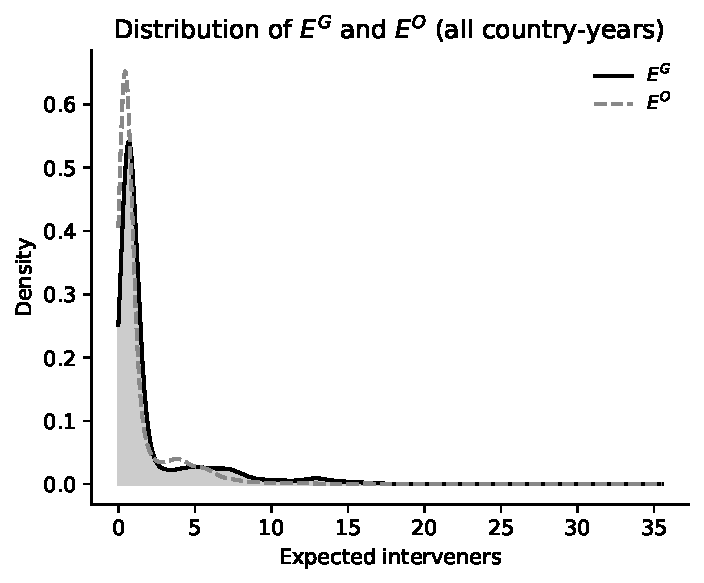
\includegraphics[width=0.85\textwidth]{fig-shadow-kde.pdf}
  \caption{Kernel density estimates of $E^G$ and $E^O$ across all
    country-years (1946--2014), averaged across 25 imputation draws.}
  \label{fig:shadow-kde}
\end{figure}

Figure~\ref{fig:shadow-ts} illustrates the temporal dynamics for three countries
with well-documented intervention environments.  South Vietnam shows the
cleanest signal: both measures ramp from approximately 0.6 in 1960 to
$E^G = 6.68$ and $E^O = 5.21$ at the peak of the war in 1972---an order
of magnitude above typical countries.
Afghanistan illustrates a regime-switching dynamic: the 1978 Saur Revolution
raises $E^G$ to 0.84, but by 1979 $E^O$ overtakes $E^G$ ($1.17$ vs $0.85$),
correctly capturing the surge in mujahideen support from Pakistan, the
United States, and others.
Egypt provides a critical out-of-sample check: it experiences no civil war
onset in our data, so the shadow measures are pure counterfactual predictions.
The classifier nonetheless tracks the geopolitical environment---the 1967
Six Day War spike ($E^G = 7.67$), the post-1972 Soviet expulsion drop, the
1991 Gulf War spike---evidence of genuine temporal tracking, not mere
onset-fitting.

\begin{figure}[t]
  \centering
  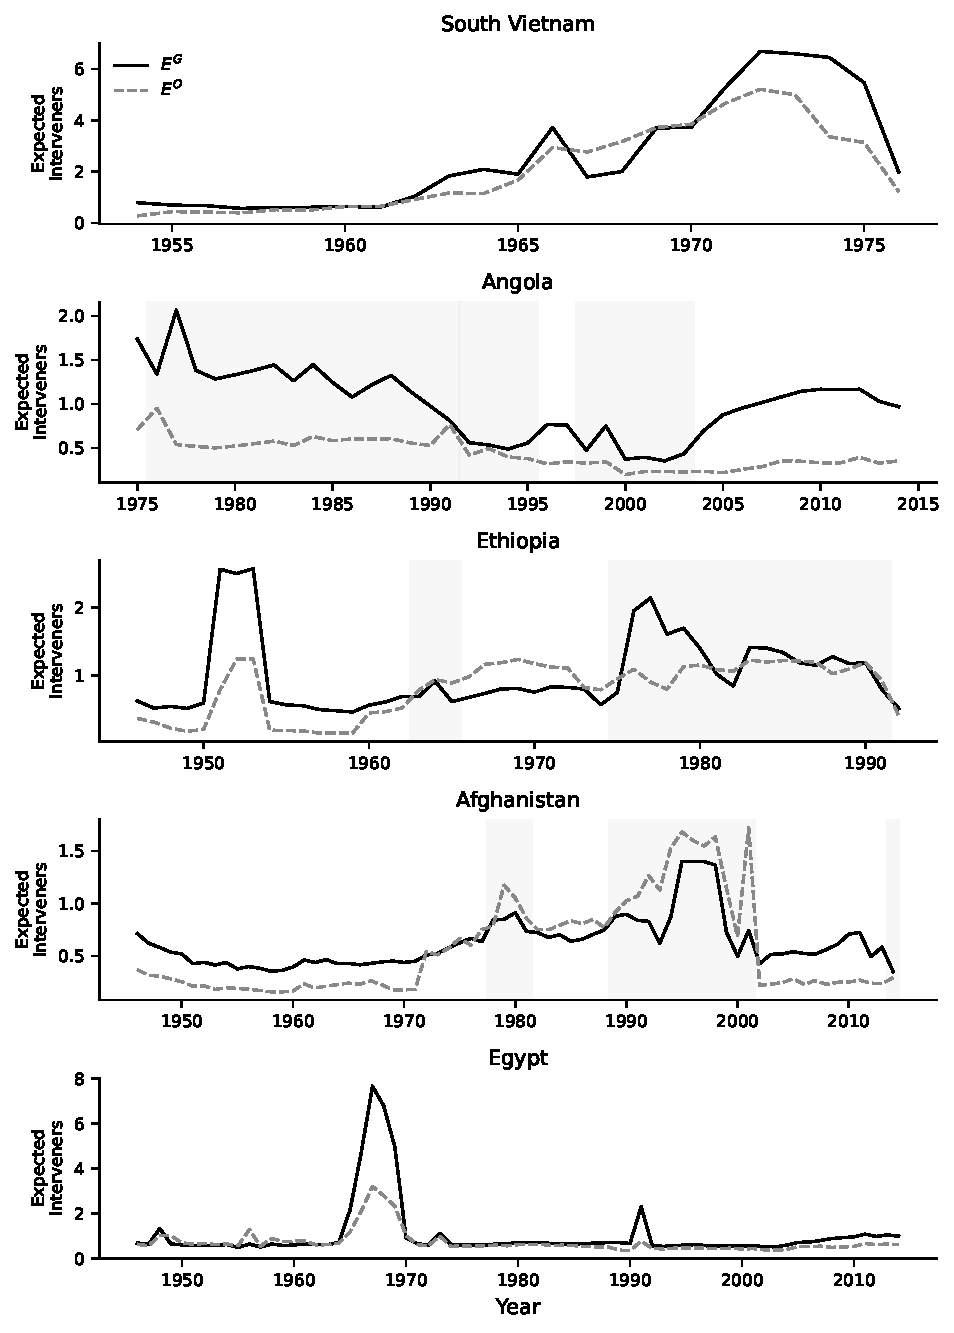
\includegraphics[width=0.85\textwidth]{fig-shadow-ts.pdf}
  \caption{Shadow measure time series ($E^G$ and $E^O$) for five countries
    with well-documented intervention environments.  Probabilities averaged
    across 25 imputation draws.}
  \label{fig:shadow-ts}
\end{figure}

$E^G$ correlates positively with both existing measures of anticipated
intervention: the Lake security hierarchy used by \citet{cunningham2016}
($r = 0.29$, $n = 161$) and the structural P5 intervention probabilities
estimated by \citet{gibilisco2022} ($r = 0.53$, $n = 145$).  The stronger
correlation with G\&M is expected---both capture intervention propensity
directly---while the moderate hierarchy correlation reflects the fact that
US dominance is only one component of the broader intervention environment
(Appendix~\ref{app:cunningham}, Figure~\ref{fig:hierarchy}).

% ============================================================
% The Decision to Fight
% ============================================================

\section{The Decision to Fight}
\label{sec:decision}

Measure in hand, I now study whether intervention expectations affect the
decision to initiate civil war.  The \textit{Entrants} model augments a standard
onset logit with the two shadow variables constructed in the previous
section:

\begin{equation*}
U_O(F; \hat{\sigma}) = \mathbf{X}\boldsymbol{\beta} + \gamma^O \sum_i \hat{\sigma}_i(O) + \gamma^G \sum_i \hat{\sigma}_i(G) + \epsilon,
\end{equation*}

\noindent where $\mathbf{X}$ contains the baseline country-year predictors and the two
summations are the expected total number of opposition-biased and
government-biased interveners, respectively.\footnote{In estimation, the
summations enter through the inverse hyperbolic sine transform,
$\operatorname{asinh}(\sum_i \hat{\sigma}_i)$, for variance stabilization.  This
introduces a concavity---diminishing marginal returns to additional
expected interveners---that is not implied by the theory.  Because
$\operatorname{asinh}$ is strictly increasing, the sign of the estimated coefficients
is invariant to this choice, and the out-of-sample model comparisons
test whether the shadow variables improve predictions regardless of
functional form.  The exact shape of the utility function over
aggregated intervention expectations is not identified from these data.}
This is the simplest
specification of Equation~\eqref{eq:EU}, in which all potential interveners carry the same
utility weight ($u_O^i(O) = \gamma^O$ and $u_O^i(G) = \gamma^G$ for
all $i$).  I relax this assumption in the heterogeneous-utilities
extensions below.

The two-stage design extends the logic of statistical backwards induction
\citep{bas2008} to an $n$-player environment.  In the two-player case, backwards
induction estimates the second mover's choice probabilities and plugs them
into the first mover's expected utility.  Here the intervention subgame
involves up to 193 simultaneous movers; separability and the Nash
fixed-point reduce the problem to one in which each intervener's marginal
probabilities suffice, and Stage~2 recovers the opposition's utility
parameters from their aggregate effect on onset.

\subsection{Empirical Strategy}

Testing these models requires a comparison point.  Following
\citet{clarke2007}, the relevant question is not whether intervention
expectations matter in isolation but whether a model that includes them
outperforms one that does not.

The \textit{Baseline} model serves as the rival.  It is a logistic regression
for civil war onset using the covariate set from
\citet{fearon2003} Table~1, Model~1---the structural
specification the literature has converged on as a reference: prior war,
log per capita income, log population, mountainous terrain, oil exporter
status, new state status, political instability, ethnic and religious
fractionalization, and democracy---estimated on our sample (COW Intra-State Wars v5.1, 1946--2014).
This is not a replication of F\&L; it is their specification used as a
comparison point on our data with updated sources.  Time-varying
covariates (income, population, democracy, political instability) are
lagged one year to avoid post-onset contamination; income and population
come from V-Dem v15 \citep{vdem2025} and democracy from the Polity project.
Civil war history is drawn from COW v5.1.  Slowly changing or fixed
characteristics---terrain, ethnic and religious fractionalization,
colonial history---are taken from the F\&L replication dataset.  To account for the mechanical growth of the summation-based
shadow variables as the state system expands, I add a year trend to all
specifications.

\citet{cederman2010} challenge the aggregate-fractionalization
baseline on the grounds that ethnopolitical exclusion from state power is
the theoretically appropriate predictor.  The Coethnics extended
specification (Section~\ref{sec:decision}) partially addresses this critique by
interacting intervention expectations with ethnic matching between the
intervener and the host country's population.

Model comparison draws on both in-sample fit and out-of-sample
predictive performance.  Within sample, I report the proportional
reduction in log-loss relative to random guessing and the area under the
ROC curve.  Out-of-sample performance uses leave-one-war-out
cross-validation: all country-years belonging to a civil war are held
out together, and predictions are formed from the remaining data.  This
scheme respects temporal dependence and avoids the information leakage
that would arise from splitting individual country-years at random.

Because the Stage~1 probabilities are estimated quantities, I retain all
25 multiply-imputed shadow measures (5 country-year imputations $\times$ 5
directed-dyad imputations) for the uncertainty analysis described below.
Point estimates for model-fit metrics are computed on the averaged shadow;
coefficient standard errors account for the full spread of measurement
draws.

\subsection{Intervention Expectations and Onset}

Table~\ref{tab:coefs} presents the paper's central result.  The two
shadow variables enter with the signs the theory requires: expected
government-biased intervention is negative ($\gamma^G = -1.62$),
consistent with deterrence, and expected opposition-biased intervention
is positive ($\gamma^O = +0.64$), consistent with emboldening.  This
directional separation holds in every one of the 25 measurement draws,
in all ten specifications reported in Table~\ref{tab:topfit}, and in the
country fixed-effects estimator.

The Entrants specification improves on the Baseline both in-sample (PRL
from 10.1\% to 11.9\%, AUC from 0.771 to 0.787) and out-of-sample
(OOS PRL = $+0.4\%$, OOS AUC from 0.650 to 0.672).  For a rare-event
model with a 2\% base rate, positive OOS PRL is a demanding bar: the
log-loss metric penalizes confident false positives severely, and the
Baseline specification---which encodes decades of accumulated knowledge
about structural onset risk---does not clear it.

\subsubsection*{Generated-Regressor Uncertainty}

Because the shadow variables are predicted from a Stage~1 classifier
rather than directly observed, standard logistic-regression errors
understate uncertainty.  \citet{knoxlucascho2022} show that this is the
most common methodological failure in learned-proxy applications: of the
48 studies they review, nearly all ignore measurement-stage variability.
I follow their recommended $T \times P$ correction: the primary analysis
runs separately for each of the $T = 25$ shadow measures, each is
bootstrapped $P = 200$ times (pairs-cluster, resampling countries), and
the resulting 5,000 coefficient vectors are pooled.

The corrected standard errors in Table~\ref{tab:coefs} are roughly
$3.5\times$ larger for $\hat{E}^G$ and $2.9\times$ larger for
$\hat{E}^O$ than naive MLE output.  A variance decomposition shows that
88--92\% of this total variance originates in the measurement
stage---variation \textit{between} shadow draws---with only 8--12\% from
primary-analysis sampling.  The measurement model, not the regression, is
the binding source of uncertainty.

Two features of the data make this unsurprising.  First, 184 onsets
across 25 measurement draws leave the Stage~2 signal thin relative to
variation in the learned proxy.  Second, $\hat{E}^G$ and $\hat{E}^O$ are
correlated at $r = 0.94$: countries that attract government-biased
intervention expectations also attract opposition-biased expectations.
This collinearity means that small perturbations in the Stage~1
classifier move both shadow variables together, inflating the
between-draw variance of each coefficient.  Tested jointly, however, the
shadow variables are unambiguous: a likelihood-ratio test rejects the
Baseline in favor of Entrants at $p < 0.001$ (LR $= 32.7$, df $= 2$),
and most type-disaggregated specifications reject Entrants in turn
(Appendix~\ref{app:lr-tests}, Table~\ref{tab:lr-tests}).  The
collinearity inflates \textit{individual} coefficient uncertainty but
does not prevent the pair from carrying strong joint signal.  The
consistent sign separation across all 25 draws---$\gamma^G < 0$ and
$\gamma^O > 0$ in every one---reinforces this: the logit reliably
separates the two effects despite having only $\approx$6\% independent
variation to work with.

Neither coefficient achieves conventional significance individually: the
95\% confidence interval for $\gamma^G$ runs from $-4.63$ to $+0.69$
and for $\gamma^O$ from $-1.94$ to $+2.59$.  Under the average
monotonicity condition of \citet{knoxlucascho2022} (\S3.1)---more of the
true intervention expectation implies more of the proxy, which the
Stage~1 calibration diagrams verify empirically
(Appendix~\ref{app:sl})---the signs of the coefficients are valid even
if the magnitudes are attenuated.  The evidence for the directional
claim therefore rests not on any single $p$-value but on the conjunction
of three facts: both coefficients carry their theoretically predicted
signs across all specifications and measurement draws; the shadow
variables improve out-of-sample prediction; and the pattern survives
country fixed effects.

Restricting Stage~2 to the labeled subsample (country-years with
observed intervention coding) yields coefficients close to the
full-sample estimates, confirming that the results are not driven by
out-of-sample extrapolation of the classifier
(\citealt{knoxlucascho2022}, \S5.6).

The fixed-effects specification (Column~3) absorbs all time-invariant
confounders---terrain, ethnic composition, colonial history---and
identifies the shadow effect from within-country temporal variation
alone.  Both coefficients retain their signs: $\gamma^G = -1.74$
(SE $= 0.47$), $\gamma^O = +0.87$ (SE $= 0.47$).  Only 71 of 171
countries exhibit variation in onset and therefore contribute to
identification.  (These standard errors are from maximum likelihood and
do not incorporate the $T \times P$ correction; they should be
interpreted as lower bounds on uncertainty.)

\begin{table}[t]
  \centering
  \begin{tabular}{@{}lrrr@{}}
    \toprule
    & Baseline & Entrants & FE Entrants \\
    \midrule
    Polity2\textsubscript{lag}         & $-$0.026 (0.014) & $-$0.032\textsuperscript{*} (0.014) & $-$0.043\textsuperscript{*} (0.019) \\
    GDP/cap (log)\textsubscript{lag}   & $-$0.670\textsuperscript{***} (0.112) & $-$0.500\textsuperscript{***} (0.122) & $-$0.232 (0.270) \\
    Pop (log)\textsubscript{lag}       & +0.110 (0.061) & +0.095 (0.066) & +0.411 (0.697) \\
    Mountainous                        & +0.223\textsuperscript{***} (0.063) & +0.126 (0.067) & \\
    Noncontiguous                      & +0.532\textsuperscript{*} (0.225) & +0.538\textsuperscript{*} (0.225) & \\
    Oil                                & +0.450\textsuperscript{*} (0.203) & +0.328 (0.208) & \\
    New state                          & +1.003\textsuperscript{**} (0.342) & +1.168\textsuperscript{**} (0.348) & +1.218\textsuperscript{**} (0.385) \\
    Instability\textsubscript{lag}     & +0.567\textsuperscript{**} (0.180) & +0.513\textsuperscript{**} (0.179) & +0.617\textsuperscript{**} (0.196) \\
    Prior war                          & +0.529\textsuperscript{**} (0.195) & +0.450\textsuperscript{*} (0.200) & $-$0.313 (0.203) \\
    Ethnic frac.                       & +0.409 (0.293) & +0.562 (0.299) & \\
    Religious frac.                    & +0.673 (0.392) & +1.225\textsuperscript{**} (0.411) & \\
    Year                               & +0.011\textsuperscript{*} (0.005) & +0.006 (0.005) & $-$0.003 (0.019) \\
    \midrule
    $\hat{E}^G$ (asinh)                &        & $-$1.62 (1.37) & $-$1.74\textsuperscript{***} (0.47) \\
    $\hat{E}^O$ (asinh)                &        & +0.64 (1.10) & +0.87 (0.47) \\
    \midrule
    Country FEs                        & No & No & Yes \\
    $N$                                & 8,792 & 8,792 & 3,750 \\
    Onsets                             & 184 & 184 & 184 \\
    PRL                                & 10.1\% & 11.9\% & \\
    AUC                                & 0.771 & 0.787 & \\
    \bottomrule
  \end{tabular}
  \caption{Logistic regression estimates for civil war onset.  Columns~1--2
    are pooled logit; Column~3 is conditional (fixed-effects) logit.
    Point estimates and standard errors for the shadow variables
    ($\hat{E}^G$, $\hat{E}^O$) in Column~2 are from a $T \times P$ bootstrap
    following \citet{knoxlucascho2022}: $T = 25$
    measurement-model draws $\times$ $P = 200$ pairs-cluster bootstrap
    replications, pooling all 5,000 coefficient vectors.  This accounts
    for uncertainty in both the Stage~1 measurement model and the Stage~2
    primary analysis.  All other standard errors are from maximum
    likelihood.  Column~3 standard errors do not incorporate the $T \times P$
    correction.  Time-invariant covariates are absorbed by country fixed
    effects in Column~3.  \textsuperscript{*}~$p < 0.05$, \textsuperscript{**}~$p < 0.01$, \textsuperscript{***}~$p < 0.001$.}
  \label{tab:coefs}
\end{table}

\subsection{Heterogeneous Utilities}

The learned-proxy approach permits a question that structural designs
cannot easily address: which types of interveners carry disproportionate
weight in the onset calculus?  The Entrants model constrains all
interveners to carry the same utility weight regardless of type.  The
theoretical framework permits the utility
parameters to vary with intervener characteristics: setting
$u_O^i(O) = \gamma_0^O + \gamma_P^O z_i$ and
$u_O^i(G) = \gamma_0^G + \gamma_P^G z_i$ for some intervener attribute
$z_i$ and aggregating produces the Entrants variables plus a pair of
type-weighted interaction terms.  I apply this to major-power status
(\textit{Powers}), geographic contiguity (\textit{Neighbors}), shared dominant ethnic
group (\textit{Coethnics}), colonial relationship (\textit{Rulers}), bilateral rivalry
(\textit{Rivals}), and military balance (\textit{DOE}).  Each type-disaggregated
specification nests the Entrants variables.

\begin{table}[t]
  \centering
  \begin{tabular}{@{}lrrrr@{}}
    \toprule
    Model & IS PRL & IS AUC & OOS PRL & OOS AUC \\
    \midrule
    Baseline       & 10.1\% & 0.771 & $-$1.0\% & 0.650 \\
    Entrants       & 11.9\% & 0.787 & +0.4\%   & 0.672 \\
    Powers         & 14.3\% & 0.809 & +1.7\%   & 0.707 \\
    Neighbors      & 14.5\% & 0.814 & +2.4\%   & 0.710 \\
    Coethnics      & 12.8\% & 0.798 & +0.4\%   & 0.680 \\
    Rulers         & 11.9\% & 0.787 & $-$0.8\% & 0.668 \\
    Rivals (bin)   & 14.4\% & 0.814 & +1.7\%   & 0.706 \\
    Rivals (cts)   & 14.7\% & 0.820 & +2.6\%   & 0.712 \\
    DOE            & 11.9\% & 0.788 & +0.2\%   & 0.671 \\
    Full           & 22.3\% & 0.866 & +4.2\%   & 0.778 \\
    \bottomrule
  \end{tabular}
  \caption{In-sample and out-of-sample fit across model specifications.
    Each extended specification nests the aggregate Entrants variables.
    IS = in-sample; OOS = leave-one-onset-group-out cross-validation.
    PRL = proportional reduction in log-loss relative to the class-frequency null.
    AUC = area under the ROC curve.}
  \label{tab:topfit}
\end{table}

Six of the nine shadow-augmented specifications outperform the Baseline
out-of-sample, with Powers, Neighbors, Rivals~(bin), and
Rivals~(cts) achieving the largest gains (OOS PRL
$\approx 1.7$--$2.6\%$, OOS AUC $\approx 0.71$), indicating that major
powers, contiguous states, and hostile dyads carry disproportionate weight
in shaping onset expectations.  The Full model achieves the highest
discriminative ability (OOS AUC = 0.778) and is the only specification
with OOS PRL above 4\%, though its 26-parameter specification risks
overfitting.

The shadow measure also subsumes the two most direct existing proxies for
anticipated intervention.  On the common sample
(6,973 country-years, 1950--2005), the Lake security hierarchy score
from \citet{cunningham2016} adds no explanatory power beyond the shadow
variables: the hierarchy coefficient is effectively zero
when the Entrants variables are included (Appendix~\ref{app:cunningham},
Figure~\ref{fig:hierarchy}).  On the 7,772 country-years where the
\citet{gibilisco2022} structural P5 intervention probabilities are
available, the pattern is the same: the G\&M aggregate score adds nothing
to the Entrants specification (LR $= 0.06$, $p = 0.80$), but the shadow
variables remain highly significant when added to a model that already
includes the G\&M score (LR $= 26.4$, $p < 0.001$).  The learned proxy
absorbs what both the hierarchy and the structural-game estimates
capture, while adding variation from non-P5 interveners, bilateral
relationships, and the spatial environment that neither alternative
covers.

% ============================================================
% Conclusion
% ============================================================

\section{Conclusion}

Civil war does not begin in a vacuum.  Opposition groups weigh the
prospect of outside military assistance against the threat of
international resistance before they decide to fight.  I have argued
that these anticipatory calculations---the shadow of intervention---
systematically shape the decision to fight, and I have developed a theory,
a measure, and an evidentiary case for that claim.

The theoretical framework embeds the onset decision in a bargain fought in
the shadow of up to $n$ potential outside powers.  Three
assumptions---separability across interveners, non-intervention as the
reference point, and a contest--burden decomposition of the war
value---reduce the opposition's calculus to a weighted sum of
intervener-specific probabilities, moving on two axes: the net tilt of the
anticipated environment and its intensity.  Worked under the common
bargaining frictions, the model signs the axes and the government channel,
declines to sign the raw opposition channel, and fixes what the evidence can
discriminate: intensity deters in every costly-war bargain, while an
emboldening tilt requires limited commitment or divergent expectations.  The
estimates then lean against the screening account as written and toward
commitment and divergent expectations, without deciding between the two.
The framework generalizes prior work by treating both directions of
intervention, the full population of potential interveners, and their
strategic interdependence.

Operationalizing this framework required constructing a measure that did
not yet exist.  The Stage~1 classifier turns a rich directed-dyad feature
set into calibrated intervention probabilities for every potential
intervener, and multiple imputation across 25 complete datasets carries
measurement uncertainty through to the final estimates.

The onset analysis returns three findings.  First, the shadow predicts.  Added
to a structural onset model, the two aggregate shadow variables improve
out-of-sample precision under leave-one-country-out cross-validation---modestly
on their own (the area under the precision--recall curve rises from
\OosBaseAucpr\ to \OosEntAucpr) and to more than double the baseline once the
shadow is resolved by intervener type (to \OosFullAucpr)---and by out-of-sample
drop-column
importance the shadow is the model's single most valuable component, above every
structural covariate.  It also subsumes the existing proxies for anticipated
intervention: neither the Lake security hierarchy \citep{cunningham2016} nor the
\citet{gibilisco2022} structural estimates adds predictive content once the
shadow is included.  Second, the shadow enters onset along the two directions on
which the mechanisms disagree: onset falls with the overall intensity of
expectations in every measurement draw and rises with the net tilt toward the
opposition in a clear majority---the two axes the collinear channels
($r \approx \CorrEgEo$) leave identified.  The pattern leans away from the standard
common-prior screen and toward limited commitment or divergent expectations,
without deciding between them; the government-biased channel, on which contest
and burden agree, is the unambiguously deterrent one.  Third, the opposition
effect, weak as a single summed expectation, is concentrated in particular
interveners and reverses sign across them: opposition backing by a neighbor or a
rival emboldens, while backing by a major power deters---a reversal I do not
press to explain here.  The undifferentiated measure was averaging these
offsetting effects away.

The results carry implications beyond the civil war literature.  The
two-stage strategy introduced here---predict the probabilities of downstream
actions, then use those predictions as regressors in a model of the
initiating decision---applies wherever a strategic choice is made in
anticipation of others' responses.  Within the civil war literature, it
supplies what the macro-correlates framework cannot: intervention
expectations shift with the decisions of specific leaders and
governments---year to year, conflict to conflict---and so carry the temporal
variation that slow-moving structural risk factors lack.

The design also speaks to the debate over machine learning's place in
quantitative political science.  \citet{grimmerrobertsstewart2021}
distinguish measurement from causal inference and name their conflation the
cardinal sin; the two stages here keep them apart---an agnostic ensemble
evaluated on predictive criteria, then a parametric onset model carrying the
inferential weight.  \citet{knoxlucascho2022} close the loop: once a proxy
is learned, its uncertainty must be propagated and its imperfections shown
not to distort conclusions.  Under their ``average monotonicity'' condition
(\S3.1)---more of the true concept implies more of the proxy, which the
Stage~1 calibration verifies---the estimated signs of the tilt and intensity
effects are valid even if the magnitudes are attenuated.

The two stages also return opposite verdicts on flexibility: the agnostic
ensemble wins Stage~1, where tens of thousands of dyad-years and
near-deterministic exclusion zones present exactly the jagged,
interaction-heavy mapping tree-based learners are built for
\citep{montgomeryolivella2018}, while the theory-shaped logit wins Stage~2,
where onsets are rare, the index is the theory's, and flexibility buys
variance with nothing left to find.  The division is the lesson: flexibility
earns its keep where data are plentiful and the truth is jagged; structure,
where events are rare and the theory supplies the functional form.

One limitation is worth stating plainly.  The analysis rests on the
Correlates of War civil war universe, the \citet{regan2000} intervention data,
and an onset specification in the \citet{fearon2003} tradition---sources that
were standard when much of this literature was built but are now dated relative
to the UCDP/PRIO Armed Conflict Dataset \citep{gleditsch2002} that anchors
contemporary civil war research.  The ACD covers a broader conflict universe
and a more recent period, and its External Support Dataset \citep{meier2023}
codes third-party involvement at a finer, actor-level granularity than the
interstate intervention record used here.  The
measurement strategy this paper develops is not tied to these particular
sources; the estimates it produces are.

Extending the approach to that data universe is a natural next step, and the
two-stage design ports directly.  Stage~1 would train the same super-learner on
ACD onset dyads, drawing intervention labels from the External Support
Dataset---whose disaggregation by support type (troops, materiel, sanctuary,
funding) would permit a richer shadow: the anticipated \textit{forms} of
involvement, not only its bias.  The Nash fixed point and the country-year aggregation carry
over unchanged; Stage~2 would regress a contemporary onset specification on the
resulting expectations, in place of the \citet{fearon2003}-style model used
here.  Two features of the ACD would sharpen the exercise: its lower
battle-death threshold admits many smaller conflicts in which intervention is
rarer, placing a premium on rare-event metrics; and its
currency through the 2010s and 2020s would bring the Syrian, Libyan, Sahelian,
and Ukrainian intervention environments within reach.  I leave this to future
work.

Whether anticipated intervention shapes the decision to fight is a substantive
question; that it can be measured---at scale, across time, and across the full
population of potential outside powers---is the prior claim on which the
answer depends.


\bibliography{references}

% ---- Online Appendix ----
\clearpage
\begin{center}
\vspace{1em}
{\Large\textbf{Online Appendix}}
\vspace{1em}
\end{center}

\appendix
% ============================================================
% Online Appendix
% ============================================================

\section{The Onset Model}
\label{app:model}

This appendix supplies the formal model behind Section~\ref{sec:motivation}.
Parts~\ref{app:game} and~\ref{app:agg} build the onset game of
Figure~\ref{fig:ntree} and derive Equation~\eqref{eq:EU}, the object the two
empirical stages estimate.  Parts~\ref{app:payoff} and~\ref{app:bargain} give
the war payoff its structure and embed it in the bargain.
Parts~\ref{app:commit}--\ref{app:diverge} work the bargain once under each of
the three common frictions; Part~\ref{app:transmit} states Expectations~1
and~2, the comparative statics Section~\ref{sec:decision} tests; and
Part~\ref{app:hetero} derives the per-type weights read by its heterogeneity
analysis.

\emph{Notation.}  $O$ and $G$ are the opposition and the government; $i = 1,
\dots, n$ indexes the potential interveners, each choosing $a_i \in \{O, N,
G\}$---back the opposition, stand aside, back the government; $\sigma_i$
collects intervener $i$'s probabilities $(\sigma_i(O), \sigma_i(G))$; $E^O =
\sum_i \sigma_i(O)$ and $E^G = \sum_i \sigma_i(G)$ are the anticipated
opposition- and government-biased intervention a country faces; $\tau = E^O -
E^G$ is the net tilt and $\iota = E^O + E^G$ the common intensity;
$\pi(\tau)$ is the contest probability and $k_O(\iota)$, $k_G(\iota)$ the war
burdens, with $k \equiv k_O$ where unambiguous; $\bar{x}$ is the
credible-concession ceiling (Part~\ref{app:commit}); $q$, $\kappa$, and $\delta(\iota)$ are the
screen's prior, resolve gap, and intensity increment
(Part~\ref{app:screen}); $\tau_O$, $\tau_G$, and $\varepsilon$ are
the two reads of the tilt and the optimism parameter
(Part~\ref{app:diverge}); and $w_i$ and $b_i$ are type-specific contest and
burden loadings (Part~\ref{app:hetero}).

\subsection{The game and its shadow}
\label{app:game}

The decision problem of Figure~\ref{fig:ntree} in the main text has three
moves.  First, the opposition $O$ chooses whether to mount a challenge; if it
does not, the status quo prevails.  Second, a challenge opens a bargain over
control of the state---a stake normalized to $1$: $O$ presses a demand $s \in
[0,1]$, which the government $G$ accepts---a settlement, on those terms---or
rejects, in which case war follows.  The bargain is worked in
Parts~\ref{app:bargain}--\ref{app:diverge}; for the game form, what matters
is that it ends in one of two ways, a settlement or a war.  Third, in war,
the $n$ potential interveners respond simultaneously---each backing the
opposition, the government, or neither---and their combined response is the
international environment in which the war is fought.

It is this third move that casts the shadow.  Because $O$ and $G$ bargain in
anticipation of how outside powers would respond, the interveners'
equilibrium response---call it $\sigma^*$---can decide between peace and war
before a shot is fired \citep{cetinyan2002}.  Interveners' payoffs depend on
the war and on one another's actions, not on the demand whose rejection
produced it, so the intervener subgame is the same at every war node and its
equilibrium $\sigma^*$ is a single, well-defined object.  Write $U_O(F)$ for
the opposition's expected payoff from a war so shaped: it is the disagreement
point of the bargain and the object the rest of this appendix works with.

\emph{Remark (rational expectations).}  Whether $\sigma^*$ approximates the
expectations that rebels actually form is not merely assumed.  Under rational
expectations, agents exploit available information at least as well as the
researcher's model \citep{muth1961}.  The Stage~1 classifier described in
Section~\ref{sec:constructing} recovers a substantial share of the predictive
content in realized intervention outcomes using only publicly observable
state characteristics; rebels who can also draw on private intelligence,
direct patron relationships, and local knowledge---and who stake their lives
on the answer---face a forecasting problem
that is easier, not harder, than the one the classifier solves.

\subsection{Aggregation}
\label{app:agg}

The shadow $\sigma^*$ is a Nash equilibrium of the intervention subgame: each
potential intervener $i$ has a utility over the profile $a = (a_1, \dots,
a_n) \in \{O, N, G\}^n$ of all interveners' actions, and at $\sigma^*$ each
plays a best response to the rest.  Stated exactly, the opposition's problem
is intractable: with every other state in the panel a potential
intervener---as many as \MaxInterveners{} in recent decades---the expected war payoff
runs over the $3^{n}$ profiles of their joint play, more than the number of
elementary particles in the observable universe.  Two assumptions reduce the
problem to a tractable form without discarding its content.

\textbf{Assumption 1 (Separability).}  The opposition's payoff from any
profile is additive across interveners: $u_O(a) = \sum_i u_O^i(a_i)$, where
$u_O^i : \{O, N, G\} \rightarrow \mathbb{R}$ measures the marginal
contribution of intervener $i$'s action.

Separability captures a specific and substantively defensible theory of how
opposition groups aggregate international expectations: each outside power's
likely behavior enters the calculus independently, and the combined effect
is their sum.  A rebel coalition assessing its international environment in
1970s Angola had a view about what Cuba would likely do, a separate view
about South Africa, and a separate view about the United States; the
hypothesis is that these entered additively.  The assumption rules out
complementarities---the value of Soviet logistics may depend on whether
Cuban troops are also present---but coordinated multilateral operations
constitute a small minority of actual interventions.\footnote{%
  \citet{aydinregan2011} find that the \textit{alignment} among interveners matters for
  civil war duration: same-side interventions shorten wars only when the
  intervening states share similar preferences.  This is evidence of
  complementarities in the conduct phase.  Separability here pertains to
  the onset calculus---the rebel's assessment of the intervention
  environment at the moment it decides whether to fight---not to the
  downstream interactions among interveners once fighting begins.  The
  spatial lags in the Stage~1 classifier (Section~\ref{sec:constructing}) capture
  interdependence among interveners' \textit{choices} without requiring that
  their \textit{effects} on the rebel enter non-additively.}

\textbf{Assumption 2 (Non-intervention as reference).}  For all $i$,
$u_O^i(N) = 0$.  This normalization makes the intervention-free onset model a
limiting case: if no state intervenes, the expected utility of fighting
reduces to purely domestic considerations, and the standard country-year
onset model follows directly.

Under these two assumptions the opposition's expected payoff from war
collapses to a sum of marginal terms.  For any joint distribution over
profiles with marginal intervention probabilities $\sigma_i$, linearity of
expectation gives $\mathbb{E}\,u_O(a) = \sum_i \mathbb{E}\,u_O^i(a_i)$, and
the standing-aside terms vanish by Assumption~2, so that
\begin{equation*}
  U_O(F; \sigma) \;=\; \sum_{i=1}^{n} \bigl[\sigma_i(O)\, u_O^i(O) +
  \sigma_i(G)\, u_O^i(G)\bigr] \tag{\ref{eq:EU}}
\end{equation*}
---Equation~\eqref{eq:EU} of the main text, here derived rather than posited.
The marginal probabilities suffice however correlated the interveners'
actions are.

That sufficiency is what carries the model to the full system of potential
interveners.  Computing the opposition's expected utility requires only the
marginals $\sigma_i$, not the joint distribution over all $n$ players'
actions simultaneously.  Specifying and estimating the full joint game---the
approach of \citet{gibilisco2022} for the five permanent Security Council
members---becomes computationally intractable beyond a small player set.
Separability sidesteps that constraint while preserving the game's central
implication: the equilibrium strategies of outside powers must be mutually
consistent.  That consistency requirement is enforced directly via the Nash
fixed-point iteration described in Section~\ref{sec:constructing}.

Equation~\eqref{eq:EU} has two kinds of unknowns---the probabilities
$\sigma_i$, estimated in Section~\ref{sec:constructing}, and the weights
$u_O^i$, recovered from onset behavior in Section~\ref{sec:decision}---and
the object of interest is the sum at the intervener equilibrium,
$U_O(F; \sigma^*)$.  The next part gives the weights their structure.

\subsection{The war payoff}
\label{app:payoff}

Two forces run through the weights $u_O^i$, and they organize everything that
follows.  The first is the \emph{contest}: support aimed at a side improves
that side's odds of prevailing.  The government-side half of this is exactly
the deterrent logic of \citet{cunningham2016}---the prospect of outside
backing for the incumbent lowers the rebels' expected return to
fighting---stated here for the full population of potential sponsors rather
than the single great-power patron on which that analysis centers.  The
second is the \emph{burden}: whichever side an entrant would favor, its
involvement makes the war it enters a bigger war---longer, heavier, harder on
the parties who must fight it.  An anticipated intervener therefore cuts
twice: once through whom the war would favor, and once through what the war
would cost.  The payoff that carries these forces is the standard one---the
opposition prevails with some probability and bears some cost,
\citeauthor{fearon1995}'s $p$ and $c$---and the shadow enters by tying each
primitive to one axis: the odds to the tilt, the burden to the intensity.

\textbf{Assumption 3 (Contest and burden).}  With $\tau \equiv E^O - E^G$
(the net tilt) and $\iota \equiv E^O + E^G$ (the common intensity), the war
payoffs, in shares of the stake, are
\[
  U_O(F) = \pi(\tau) - k_O(\iota), \qquad
  U_G(F) = \bigl(1 - \pi(\tau)\bigr) - k_G(\iota),
\]
where the contest probability $\pi$ is increasing in the tilt, each burden
$k_O$, $k_G$ is increasing in the intensity, and all three are affine over
the observed range; states expected to stand aside add no burden (the
normalization of Assumption~2).  Where only the opposition's burden is in
play, write $k \equiv k_O$ and $k' \equiv k_O'$.

Assumption~3 states the war payoff in aggregate coordinates;
Equation~\eqref{eq:EU} requires it to be additive across interveners with
fixed marginal weights.  Affinity is what reconciles the two.  Because
$\pi$ and $k_O$ are affine, each can be written exactly as its intercept plus
a constant slope, $\pi(\tau) = \pi(0) + \pi'\tau$ and $k_O(\iota) = k_O(0) +
k'\iota$.  Substitute the definitions $\tau = E^O - E^G$ and $\iota = E^O
+ E^G$, with $E^O = \sum_i \sigma_i(O)$ and $E^G = \sum_i \sigma_i(G)$:
\begin{align*}
  U_O(F) &= \pi(\tau) - k_O(\iota) \\
  &= \bigl[\pi(0) - k_O(0)\bigr] + \pi'\,\bigl(E^O - E^G\bigr)
     - k'\,\bigl(E^O + E^G\bigr) \\
  &= \bigl[\pi(0) - k_O(0)\bigr] + \sum_{i=1}^{n}
     \Bigl[(\pi' - k')\,\sigma_i(O) \;-\; (\pi' + k')\,\sigma_i(G)\Bigr].
\end{align*}
The sum is Equation~\eqref{eq:EU}, with the same pair of marginal weights for
every intervener,
\[
  u_O^i(O) = \pi' - k', \qquad u_O^i(G) = -(\pi' + k');
\]
a curved $\pi$ or $k$ would instead make intervener $i$'s marginal
contribution depend on the rest of the environment, breaking the additive
form.  The bracketed intercept $\pi(0) - k_O(0)$ is the war value absent
any anticipated intervention---the purely domestic term of Assumption~2's
reference point---constant in the shadow and absorbed empirically into the
second stage's domestic baseline $\mathbf{X}\boldsymbol{\beta}$;
Equation~\eqref{eq:EU} records the shadow-dependent part, through which every
derivative below runs.  Two readings follow at once.  On the government side
the two forces agree: backing for the incumbent worsens the rebels' odds
\emph{and} heightens the war's burden, so the theory signs that channel
unambiguously, $-(\pi' + k') < 0$.  On the opposition side they compete:
outside backing improves the rebels' odds but heightens the burden of the
very war in which the help would arrive, and $\pi' - k'$ is a race the theory
does not resolve.  The natural coordinates of the war payoff are therefore
not the two channels but the two axes---the tilt, which moves the contest,
and the intensity, which moves the burden---the combinations the second-stage
analysis can estimate with any stability (Section~\ref{sec:decision}).

\emph{Remark (why affine).}  Affinity is a local claim, and four observations
bound its cost.  The observed tilt spans a short arc---the second stage's
tenth-to-ninetieth-percentile move covers well under a unit on the asinh
scale---over which any smooth contest function is approximated by its chord.
The tilt is a difference of matched, co-moving aggregates, so it operates in
the interior of any S-shaped contest function, where curvature is
second-order.  The estimation scale is already concave in raw counts---the
channels enter through asinh---so affinity in $\tau$ still embodies
diminishing returns to additional interveners.  Affinity is also exactly
mean-shadow sufficiency, $\mathbb{E}[\pi(\tau)] = \pi(\mathbb{E}\tau)$:
without it the shadow's variance, not just its level, would become
payoff-relevant, and the measure would owe the reader second moments.  And
the conclusions do not hang on it: the next Remark shows the channel signs
survive on monotonicity alone, and the interaction probe of
Part~\ref{app:commit} turns up none of the negative tilt-by-intensity product a
scaling burden would imply.

\emph{Remark (general form).}  Nothing below turns on the exact separation of
contest from burden in Assumption~3.  With a general $\pi(E^O, E^G)$, increasing in $E^O$ and
decreasing in $E^G$, and a general $k(E^O, E^G)$, weakly increasing in both,
the channel-coordinate conclusions hold unchanged---$\partial U_O(F)/\partial
E^G = \pi_{E^G} - k_{E^G} < 0$ always, while $\partial U_O(F)/\partial E^O =
\pi_{E^O} - k_{E^O}$ is unsigned---and the axis conclusions hold iff direction
moves the contest more than the burden, $\pi_{E^O} - \pi_{E^G} > k_{E^O} -
k_{E^G}$, and intensity moves the burden more than the contest, $k_{E^O} +
k_{E^G} > \pi_{E^O} + \pi_{E^G}$; both are automatic under the separated form.
The empirical mapping is a rotation, not a test: the second stage's axis
coefficients estimate $(\pi', -k')$ directly.  Two overidentifying
inequalities do follow for the raw channels---the government-side effect
exceeds the opposition-side effect in magnitude, $\pi' + k' > |\pi' - k'|$,
and it exceeds the intensity effect, $-(\pi' + k') < -k' < 0$---and both hold
in the estimates of Section~\ref{sec:decision}.

\subsection{The bargaining stage}
\label{app:bargain}

Now embed the war value in the bargain.  The protocol is the game's second
move: on challenging, $O$ presses its demand $s \in [0,1]$ (its share; $G$
keeps $1 - s$), which $G$ accepts---ending in peace---or rejects, in which
case war follows.  $G$ accepts iff $1 - s \ge U_G(F)$, that is, iff
\begin{equation}
  s \le \pi(\tau) + k_G(\iota). \label{eq:accept}
\end{equation}

Absent any friction the bargain never breaks.  The largest demand $G$
accepts, $s = \pi + k_G$, exceeds $O$'s war payoff $\pi - k_O$ by the joint
burden $k_O + k_G > 0$, so $O$ demands exactly that, $G$ accepts, and war
never occurs---neither axis moves onset, because onset never varies.  The
three parts that follow restore one friction at a time---a commitment
ceiling, private resolve, divergent reads of the shadow---each in the
vocabulary of Assumption~3.

\subsection{The commitment cutpoint}
\label{app:commit}

Suppose first that the war costs are common knowledge but that $G$ cannot
credibly transfer more than a share $\bar{x} < 1$ of the stake: it cannot bind
its later self to honor a larger concession once the external threat recedes.
Feasible peaceful offers are then those with $s \le \bar{x}$.  Since $O$
accepts no share below its war payoff $U_O(F)$, a peaceful division exists iff
$U_O(F) \le \bar{x}$, and war---onset---occurs exactly when
\begin{equation}
  U_O(F) = \pi(\tau) - k_O(\iota) > \bar{x}. \label{eq:cutpoint}
\end{equation}
(When the ceiling blocks peace it is the ceiling, not $G$'s willingness, that
blocks it: $U_O(F) \le \pi + k_G$ always, so a demand $G$ would accept exists
but exceeds what $G$ can credibly deliver.)  Because $\pi$ rises in the tilt
and $k_O$ in the intensity, \eqref{eq:cutpoint} is a cutpoint: holding the rest
fixed, onset switches on as the tilt rises and off as the intensity rises.
Across a population of country-years with heterogeneous $(\bar{x}, k_O)$, the
probability of onset is
$\Pr\!\big(\pi(\tau) - k_O(\iota) > \bar{x}\big)$---a smooth function
increasing in the tilt, decreasing in the intensity, and saturating in $\pi \in
[0,1]$, the form the second-stage link estimates, with unobserved
heterogeneity in the threshold as its error (the domestic intercept
$\pi(0) - k_O(0)$ and the threshold's observable movers are the second
stage's $\mathbf{X}\boldsymbol{\beta}$).\footnote{The additive form of \eqref{eq:cutpoint} carries a testable implication: a burden that \emph{scaled} the contest rather than adding to it would sign a tilt-by-intensity product term negative on the index scale. Re-estimating the second-stage model with that product term returns no such negative sign---the coefficient is instead weakly positive (positive in \DirInterFrac\ percent of the 25 measurement draws), so the scaling variant is disfavored. The interaction is not sharply estimated in either direction, as one expects of a product of two channels that are themselves nearly collinear, and none of the paper's claims depends on its form.}

The tilt relationship is weakly monotone, never sign-reversing, provided the
credible ceiling does not rise with the tilt faster than the contest does:
$\partial \bar{x}/\partial \tau < \pi'$ suffices for single crossing of
\eqref{eq:cutpoint} in $\tau$.
This is precisely where the account parts from \citet{lango2023}, who shows
that anticipated opposition-biased intervention can \emph{lower} onset: by
tipping the balance of power against the government, it compels some
governments to acquiesce---to concede power outright---rather than fight.
That pacifying channel runs through \emph{credible} concession, modeled there
as a terminal transfer of power; the commitment friction is precisely its
denial---the assumption that credible concession is bounded and does not grow
with the opposition's external backing.  The two accounts agree on what is at
issue and part only there.  We adopt the friction, and the data lean its
way: the tilt of the anticipated environment toward the opposition
predicts \emph{more} onset, not less
(Section~\ref{sec:decision}).\footnote{The qualitative record agrees the net
pull is toward war, with rebel leaderships documented conditioning the
decision to fight on anticipated outside support \citep{kuperman2008,
kyddstraus2013}.}

\subsection{The common-prior resolve screen}
\label{app:screen}

Now drop the ceiling and restore the standard information friction: $G$'s
resolve is private.  The bargain that results is the ubiquitous ultimatum
screen \citep[e.g.,][]{slantchevtarar2011}, transposed to the onset setting.  $G$ is resolute or soft: the resolute type bears only
the common intensity burden $\delta = \delta(\iota)$ that war imposes on
every combatant ($O$'s war cost is $k_O + \delta$; the setup's $k_O(\iota)$
thus decomposes as an intensity-free base plus the common increment), while
the soft type bears an additional resolve gap $\kappa > 0$; $q \equiv
\Pr(\text{resolute})$ is common knowledge.  By \eqref{eq:accept} the resolute
type accepts any demand $s \le \pi + \delta$ and the soft type any $s \le \pi
+ \kappa + \delta$, so the soft type accepts more.  Two pure demands are
undominated.  The \emph{safe} demand $s = \pi + \delta$ is accepted by both
types and yields $O$ that amount with certainty.  The \emph{risky} demand
$s = \pi + \kappa + \delta$ is accepted only by the soft type: with
probability $1 - q$ it yields $\pi + \kappa + \delta$, and with probability
$q$ it is refused and war yields $U_O(F) = \pi - k_O - \delta$.  $O$ prefers
the risky demand iff
\[
  (1 - q)(\pi + \kappa + \delta) + q(\pi - k_O - \delta) \;\ge\; \pi + \delta,
\]
which reduces to
\begin{equation}
  (1 - q)\,\kappa \;\ge\; q\,(k_O + 2\delta). \label{eq:riskreturn}
\end{equation}
Two things have happened.  The balance of power $\pi(\tau)$ has dropped out:
it shifts both acceptance thresholds and $O$'s war payoff by the same amount,
relocating the division but cancelling from the risky-versus-safe comparison.
The burden has not: $\delta(\iota)$ survives on the right of
\eqref{eq:riskreturn}---the war $O$ risks is costlier, while the safe demand,
tracking both types' diminished war values, extracts more---so the
equilibrium probability of war,
\[
  \Pr(\text{onset}) = q \cdot \mathbf{1}\!\left[(1 - q)\,\kappa \ge
  q(k_O + 2\delta)\right],
\]
is weakly \emph{decreasing} in the intensity and independent of the tilt.  At the
corner, where $\pi$ is high enough that demands are capped at the whole stake,
raising $\pi$ only \emph{lowers} the chance of war, as $O$ comes to extract
the entire stake peacefully; the screen therefore never produces a positive
tilt effect, interior or corner.

Two features of the cost structure are load-bearing.  The intensity increment is
\emph{additive} and \emph{type-common}: it attaches to the character of the
war---longer, heavier, more internationalized---rather than to the
government's resolve.  A multiplicative burden scaling all costs equally would
cancel from the interior comparison, and an increment that fell
disproportionately on the soft type could reverse the sign; the substantive
content of Assumption~3's burden is exactly the type-common reading.

\emph{Remark (screening on capacity).}  Nothing here turns on resolve being
the private object.  Let the government's type instead be its capacity: $O$
prevails with probability $\pi_L(\tau)$ against a strong government and
$\pi_H(\tau)$ against a weak one, $\pi_H(0) > \pi_L(0)$, both types shifted
equally by the tilt, with the war costs $k_O + \delta$ and $k_G + \delta$
common knowledge.  The screen replays: the weak type accepts more, the safe
demand is $\pi_L + k_G + \delta$, and the risky demand $\pi_H + k_G + \delta$
is refused by the strong type---against whom the war is then fought.  The
risky demand is preferred iff
\[
  (1 - q)\,\Delta\pi \;\ge\; q\,(k_O + k_G + 2\delta), \qquad
  \Delta\pi \equiv \pi_H(0) - \pi_L(0),
\]
with $q$ now the probability of the strong type.  The tilt enters the safe
demand, the risky demand, and the war payoff alike, and cancels with weights
$(1 - q) + q - 1 = 0$; the intensity survives in $2\delta$.  The row is
unchanged: what is screened supplies the spread---the resolve gap $\kappa$ or
the capacity gap $\Delta\pi$---but the cancellation belongs to the screen
itself, so a positive tilt effect excludes it whatever the private object.
(As with costs, type-dependence in the \emph{sensitivity} to the tilt,
$\pi'_H > \pi'_L$, would let the spread grow with $\tau$ and transmit it; the
parallel caveat applies.)

The screen, then, transmits the intensity and blocks the tilt: onset falls in
$\iota$ here as under commitment, but no positive tilt effect can arise
through this channel.  It is the tilt's presence in the data, not the
intensity's, that discriminates among the frictions (Expectation~2, Part~\ref{app:transmit}).

\subsection{Divergent expectations}
\label{app:diverge}

Finally, drop the private resolve and let the parties read the shadow itself
differently.  The shadow is a forecast of third parties' conduct in a war that
has not happened; no pre-war exchange can realize it, so the government and
the rebels can hold---and know they hold---different estimates of it
\citep{cetinyan2002, thyne2006}.%
% CITE-SLOT (updated 2026-07-15): Fey & Ramsay 2007 READ + CITED (Theorem 1, common-prior no-war). Slantchev & Tarar 2011 READ + CITED (common-prior processing point, clause below) + aumann1976 added (verified via S&T ref list). OPTIONAL remaining: Smith & Stam 2004 (heterogeneous-priors war model) — still not in readings/; do not add unverified.
{}  Held as common knowledge, such divergence departs from common priors
\citep{aumann1976}: among common-prior rationals, different reads are private
information, and the bargain processes private information as the
screen \citep[cf.][]{slantchevtarar2011}.  This friction therefore runs on
priors that differ---a primitive the other two bargains do not need.  Let
$\tau_O$ and $\tau_G$ be the two reads of the tilt, common
knowledge, with war costs $k_O(\iota)$ and $k_G(\iota)$ as above.  $G$ accepts
any demand $s \le \pi(\tau_G) + k_G$, and $O$, knowing this, compares the best
acceptable settlement with war as \emph{it} sees war: onset occurs iff
$\pi(\tau_O) - k_O > \pi(\tau_G) + k_G$, that is, iff
\begin{equation}
  \pi(\tau_O) - \pi(\tau_G) \;>\; k_O(\iota) + k_G(\iota).
  \label{eq:wedge}
\end{equation}
War requires the rebels' optimism about the tilt to exceed the joint burden of
fighting.  Under proportional optimism---$\tau_O = (1+\varepsilon)\tau$,
$\tau_G = \tau$, $\varepsilon > 0$---the wedge is $\varepsilon \pi' \tau$,
growing wherever the environment tilts toward the opposition; across
country-years heterogeneous in $(\varepsilon, k_O + k_G)$, the probability of onset
rises in $\tau$ (on $\tau > 0$) and falls in $\iota$.  Two limits mark the
channel's shape: it is one-sided, silent where the environment tilts against
the opposition, and it saturates, the wedge vanishing as $\pi$ approaches its
bounds.  Under a common prior the construction would unravel: because war here
requires both a demand the government will refuse and the refusal itself,
each side must read the other's willingness to fight as information, and
\citet{feyramsay2007} show that no equilibrium war survives those
inferences---war by mutual optimism requires beliefs a common prior cannot
deliver.  The channel therefore rests on heterogeneous priors, and what makes
that escape unusually defensible here is the object of the disagreement: the
counterfactual conduct of third parties, which no pre-war exchange between
the combatants can arbitrate and only war itself reveals.  This is the mechanism of
\citet{cetinyan2002} and \citet{thyne2006} in the present notation: not the
potential for intervention but different expectations of it is what moves
onset through this channel.

\subsection{What the frictions transmit}
\label{app:transmit}

The three instances work the bargain once under each friction, all in the
vocabulary of Assumption~3, and their comparison yields a taxonomy: the two
axes carry different evidentiary weight.  That onset falls with the intensity
of the anticipated environment is close to common property---any costly-war
bargain that produces war with positive probability delivers it.  That onset
rises with the tilt is the diagnostic fact: no frictionless or common-prior
account transmits it, so its presence in the data is a trace of a friction
that lets the balance of power reach the decision to fight.

\textbf{Expectation 1 (Axes of the shadow).}  Under the commitment friction,
the probability of onset is increasing in the net tilt $\tau = E^O - E^G$ and
decreasing in the common intensity $\iota = E^O + E^G$ of anticipated
intervention (by Equation~\eqref{eq:cutpoint} and the weights of
Part~\ref{app:payoff}).  In channel coordinates the government-side effect is
$-(\pi' + k') < 0$---contest and burden push together---while the
opposition-side effect is the race $\pi' - k'$, which the theory does not
sign.  The account is falsified by a robustly negative tilt effect or a
robustly positive intensity effect; it is falsified by neither sign of the
raw opposition channel, whose fragility it expects.

\textbf{Expectation 2 (What the frictions transmit).}  The probability of
onset falls in the common intensity under all three bargains---weakly under
the common-prior screen, strictly under the commitment ceiling and divergent
expectations---but rises in the net tilt only under the latter two: under
commitment throughout, under divergent expectations one-sidedly, on the
region where the environment already tilts toward the opposition.  Under the
common-prior screen it cannot rise in the tilt, interior or corner.  A
positive tilt effect therefore excludes the frictionless and common-prior
accounts, while leaving commitment and divergent expectations in contention;
a negative intensity effect is common property, diagnostic of the burden
rather than of any friction.

\medskip
\begin{center}
  \small
  \begin{tabular}{@{}lccc@{}}
    \toprule
    & \multicolumn{2}{c}{Effect on $\Pr(\text{onset})$ of} & \\
    \cmidrule(lr){2-3}
    Bargain & tilt $\tau$ & intensity $\iota$ & Derived at \\
    \midrule
    Frictionless & \multicolumn{2}{c}{none: war never occurs} & Part~\ref{app:bargain} \\
    Common-prior screen & $0$ interior; $\le 0$ at corner & $-$ (weakly) & \eqref{eq:riskreturn} \\
    Commitment ceiling & $+$ & $-$ & \eqref{eq:cutpoint} \\
    Divergent expectations & $+$ on $\tau > 0$; silent on $\tau \le 0$ & $-$ & \eqref{eq:wedge} \\
    \bottomrule
  \end{tabular}
\end{center}
\medskip

The exclusion is of the screen as written.  The load-bearing caveats of
Part~\ref{app:screen} mark the escape routes---a burden that scales rather
than adds, an increment that falls disproportionately on the soft type,
type-dependent sensitivity to the tilt---and a screening variant built along
any of them is a legitimate rival, testable against data richer than these.

Onset data cannot separate the two surviving frictions, and we do not ask
them to.  We lead with commitment for its prominence across the civil-war
record, its aptness to military intervention, where the calculus of
victory really is altered \citep{walter2009}, and its economy of
primitives: the ceiling's source is ready-made---settle, the external threat
recedes, and with it whatever concession it extracted
(Part~\ref{app:commit})---while divergence runs on the differing priors
Part~\ref{app:diverge} must posit \citep{aumann1976}.  The
divergent-expectations reading remains a live alternative rather than a
rival.

\subsection{Heterogeneous interveners}
\label{app:hetero}

One more consequence of Equation~\eqref{eq:EU} is worth setting down, because
Section~\ref{sec:decision} uses it.  Nothing in Assumption~1 requires the
weights to be uniform across interveners; uniformity entered with
Assumption~3's unweighted aggregates.  Generalize them: let $w_i \ge 0$ and
$b_i \ge 0$ be type-specific contest and burden loadings---how much
intervener $i$'s entry would move the balance, and how much it would
internationalize the war---and let
\begin{gather*}
  U_O(F) = \pi(\tau_w) - k(\iota_b), \\
  \tau_w \equiv \sum_i w_i\bigl[\sigma_i(O) - \sigma_i(G)\bigr], \qquad
  \iota_b \equiv \sum_i b_i\bigl[\sigma_i(O) + \sigma_i(G)\bigr].
\end{gather*}
The weighted aggregator is the assumption; the per-type weights are its
arithmetic.  Expanding as before, $u_O^i(O) = \pi' w_i - k' b_i$ and
$u_O^i(G) = -(\pi' w_i + k' b_i)$, with Assumption~3 the case $w_i = b_i =
1$.  The government-side weight is nonpositive for every type, strictly
negative wherever either loading is positive: no anticipated intervener
emboldens rebellion from the government's side.  The opposition-side race, by
contrast, may resolve differently for different interveners: a state whose
involvement would internationalize the war more than tilt it ($k' b_i > \pi'
w_i$) deters even from the opposition's side---the signature
Section~\ref{sec:decision} reads in the major-power reversal.  The theory
fixes the aggregate axes and the government channel; which interveners carry
which weight is a question for measurement.

\emph{Remark (what the model stakes).}  Three limits are built into the
empirical exercise this model serves.  The shadow is estimated, not observed,
so effect magnitudes arrive blurred by measurement error; its two channels
co-move tightly, so only their sum and difference are stable; and the
observable is onset, not the terms of the settlements that avert it, so the
friction is detectable only through its trace.  The model is pitched at the
altitude of signs deliberately---strong enough that a reversed sign would
falsify it, no stronger than the measurement can carry.  And no claim is made
that any one of these games is \emph{the} mechanism: the pair of comparative
statics is what any account with a monotone contest, an intensity-borne
burden, and either surviving friction implies.

\section{Regan Intervention Coding Corrections}
\label{app:coding}

The raw \citet{regan2000} data contain ten per-conflict coding decisions that are
corrected before analysis.  These are listed in
Table~\ref{tab:regan-corrections}.  In all cases the corrections are applied to the raw
Stata file \textit{before} country-code standardization, matching the original R
pipeline's order of operations.

\begin{table}[t]
  \centering
  \footnotesize
  \begin{tabular}{@{}p{3cm}lp{3cm}p{4.5cm}@{}}
    \toprule
    \textbf{Conflict} & \textbf{State} & \textbf{Correction} & \textbf{Rationale} \\
    \midrule
    Congo-Brazzaville (1997) & France (220) & target: neutral $\to$ 2 (opp) & France supplied arms to Cobra militia, siding with Angola/opposition \\
    Indonesia (1958) & USA (002) & target: gov $\to$ 2 (opp) & CIA Operation Archipelago backed anti-communist rebels \\
    Cameroon (conflict 17) & W.\ Germany & ccode: 255 $\to$ 260 & Miscoded; correct COW code for West Germany \\
    Congo Crisis (1960s) & All & host ccode: 484 $\to$ 490 & DRC better represents this conflict than Republic of Congo \\
    Congo Crisis (1964) & Belgium (211) & target flipped gov$\leftrightarrow$opp & Sides effectively reversed in 1964 phase \\
    Ethiopia (1980s) & Somalia (520) & target: gov $\to$ 2 (opp) & Somalia generally supported Ogaden opposition \\
    Cambodia & Vietnam (816) & target: opp $\to$ 1 (gov) & Vietnam supported incumbent government throughout \\
    Mozambique & Zimbabwe (552) & target: $\to$ 1 (gov) & Zimbabwe consistently backed FRELIMO government \\
    Mozambique & Malawi (553) & target: $\to$ 3 (neutral) & Malawi supported both sides; excluded as neutral \\
    Zimbabwe/South Africa & South Africa & target: $\to$ 3 (neutral) & Supported both sides; excluded \\
    Sri Lanka & UK (200) & target: $\to$ 2 (opp) & Miscoded; correct side assignment \\
    Sri Lanka & India (750) & target: $\to$ 1 (gov) & India supported government \\
    Iran & Iraq (645) & target: gov $\to$ 1 & Iraq favored government; miscoded in original \\
    \bottomrule
  \end{tabular}
  \caption{Regan coding corrections applied before analysis.}
  \label{tab:regan-corrections}
\end{table}

After corrections, two directed dyads with conflicting target assignments across
multiple records are resolved by fixing the target directly: Georgia--Russia
(opposition-biased) and Liberia--Sierra Leone (government-biased).  Final
deduplication retains the first record per directed dyad-year after sorting by
the \texttt{ddyear} identifier.

\subsection{Post-1999 Intervention Coding}
\label{app:post1999}

The \citet{regan2000} data end in 1999.  To extend the Stage~1 training set through 2014,
I code military interventions in all 38 post-1999 COW onset country-years using the
same threshold: deployment of military personnel (troops, combat advisors, or
directed proxy forces) attributable to a specific state, on behalf of one side.
Arms transfers, economic aid, sanctuary, and strategic direction alone are
insufficient.  UN peacekeeping missions are excluded.  Table~\ref{tab:post1999} lists
the 32 coded interventions; the remaining 17 onset country-years are coded as
having no intervention meeting the threshold.  Full source notes for each
coding decision are available in the replication archive.

\begin{table}[p]
  \centering
  \footnotesize
  \begin{tabular}{@{}llll@{}}
    \toprule
    \textbf{Host} & \textbf{Year} & \textbf{Intervener} & \textbf{Side} \\
    \midrule
    Sierra Leone   & 2000 & United Kingdom  & Gov. \\
    Ivory Coast    & 2002 & France          & Gov. \\
    Liberia        & 2002 & Guinea          & Opp. \\
    Pakistan       & 2004 & United States   & Gov. \\
    Chad           & 2005 & France          & Gov. \\
    Chad           & 2005 & Sudan           & Opp. \\
    Pakistan       & 2005 & United States   & Gov. \\
    Somalia        & 2006 & Ethiopia        & Gov. \\
    Chad           & 2007 & France          & Gov. \\
    Chad           & 2007 & Sudan           & Opp. \\
    Pakistan       & 2007 & United States   & Gov. \\
    Somalia        & 2009 & Ethiopia        & Gov. \\
    Iraq           & 2010 & United States   & Gov. \\
    Ivory Coast    & 2011 & France          & Opp. \\
    Libya          & 2011 & United States   & Opp. \\
    Libya          & 2011 & United Kingdom  & Opp. \\
    Libya          & 2011 & France          & Opp. \\
    Libya          & 2011 & Qatar           & Opp. \\
    Libya          & 2011 & UAE             & Opp. \\
    Mali           & 2012 & France          & Gov. \\
    Mali           & 2012 & Chad            & Gov. \\
    Nigeria        & 2013 & Chad            & Gov. \\
    South Sudan    & 2013 & Uganda          & Gov. \\
    Ukraine        & 2014 & Russia          & Opp. \\
    Somalia        & 2014 & Ethiopia        & Gov. \\
    Somalia        & 2014 & Uganda          & Gov. \\
    Libya          & 2014 & Egypt           & Gov. \\
    Libya          & 2014 & UAE             & Gov. \\
    Yemen          & 2014 & Saudi Arabia    & Gov. \\
    Yemen          & 2014 & UAE             & Gov. \\
    Afghanistan    & 2014 & United States   & Gov. \\
    Afghanistan    & 2014 & United Kingdom  & Gov. \\
    \bottomrule
  \end{tabular}
  \caption{Post-1999 military interventions in COW onset country-years.
    Gov.\ = government-biased; Opp.\ = opposition-biased.}
  \label{tab:post1999}
\end{table}

Onset country-years coded as having no military intervention meeting the
personnel-deployment threshold: Guinea (2000), Philippines (2000, 2003, 2005),
Burundi (2001), Rwanda (2001), Nepal (2001, 2003), Sudan (2003, 2011),
Indonesia (2003), Yemen (2004, 2007), Sri Lanka (2006), Syria (2011),
Myanmar (2011), and Central African Republic (2012).

\section{Multiple Imputation Procedure}
\label{app:imputation}

Missing values in continuous predictors are handled through a two-stage
multiple imputation strategy using miceforest (Multiple Imputation by Chained
Equations with LightGBM).  The strategy generates $5 \times 5 = 25$ complete
datasets; estimates are combined across datasets following \citet{rubin1987}.

The staged structure reflects the data's own hierarchy and is a design
choice, not a computational convenience.  Country-year quantities (GDP per
capita, regime scores, CINC components) must be imputed at the country-year
level: imputing them at the directed-dyad level would treat state $A$'s GDP
as a separate quantity in each of $A$'s dyads, producing inconsistent imputed
values across rows that share the same country and year.  Dyadic quantities
(bilateral trade, peace scores, capital distances) must be imputed before
directed expansion so that the symmetry constraint $x_{AB} = x_{BA}$ holds
within each imputed dataset---a constraint that would be broken if each
directed-dyad row were imputed independently.  Imputing in sequence,
country-year first and undirected dyad second, preserves both requirements
simultaneously.

\textbf{Stage~1---Country-year imputation.}  The analysis sample (1946--2014, $n =
8{,}897$ country-years) is imputed five times.  Variables imputed include
regime scores, GDP per capita, population, oil wealth, mountainous terrain,
ethnic fractionalization, ethnic exclusion, all six NMC capability components,
and UN ideal points.  Six right-skewed NMC variables are asinh-transformed
before imputation (with individually optimised scale parameters minimising the
Kolmogorov--Smirnov statistic against the standard normal) and back-transformed
afterwards.  Five iterations of chained equations are run.  Post-imputation
clipping enforces substantive constraints ($-10 \leq$ \texttt{polity2} $\leq 10$,
probabilities $\in [0,1]$, capabilities $\geq 0$).

\textbf{Stage~2---Undirected-dyad imputation.}  For each of the five country-year
datasets, the undirected dyad frame (${\sim}$599,000 rows) is imputed five times before
expansion to directed dyads.  Imputation at the undirected-dyad stage ensures
that symmetric quantities (trade flows, peace scores, capital distance) satisfy
$x_{AB} = x_{BA}$ by construction within each imputed dataset.  Variables
imputed include bilateral trade flows, peace quality scores, capital distances,
and dispute outcome expectations.  Two iterations of chained equations are run.

The 25 resulting complete datasets are processed identically through the
spatial-weights and intervention-coding stages before combination.\footnote{%
  The 25 branches are mutually independent at every stage upstream of the
  final combination: each (cy, ud) pair flows from imputation through
  Stage~1 training, Stage~1 prediction, and Stage~2 estimation without
  reference to any other branch.  Rubin's Rules averaging is the only step
  that requires all 25 to be complete.  This means the pipeline is
  embarrassingly parallel---all 25 classifiers could in principle be trained
  simultaneously---and that updating the sample in a future study would not
  require retraining all 25 models from scratch.  A single additional
  imputed dataset, processed through the same pipeline, contributes
  marginally to the final combination.}

\section{Variable List}
\label{app:varlist}

Feature sources: material capabilities from COW v6 \citep{singer1987}
and V-Dem v15 \citep{vdem2025}; ethnic structure from
\citet{fearon2003} and \citet{cederman2010}; alliances
\citep{gibler2009}; contiguity \citep{stinnett2002}; territorial
disputes \citep{huth2003}; expected dispute outcomes
\citep{carroll2019}; peace quality \citep{diehl2019}; UN General
Assembly ideal points \citep{bailey2017}; and IGO membership
\citep{pevehouse2020}.

Table~\ref{tab:cy-vars} lists all country-year variables included in the analysis.
Table~\ref{tab:dyad-vars} lists the dyadic variables added at the directed-dyad stage.

\begin{table}[p]
  \centering
  \scriptsize
  \begin{tabular}{@{}lp{5cm}ll@{}}
    \toprule
    \textbf{Variable} & \textbf{Description} & \textbf{Source} & \textbf{Coverage} \\
    \midrule
    \texttt{onset} & Civil war onset (COW types 4--5, $\geq$ 1,000 battle deaths) & COW ISW v5.1 & 1946--2014 \\
    \texttt{polity2} & Polity II score ($-10$ to $+10$) & V-Dem v15 (\texttt{e\_polity2}) & 1946--2014 \\
    \texttt{v2x\_polyarchy} & Electoral democracy index (0--1) & V-Dem v15 & 1946--2014 \\
    \texttt{instab} & Political instability (large Polity swing or coup) & V-Dem v15 & 1946--2014 \\
    \texttt{lgdp} & Log GDP per capita (2011 PPP int'l \$) & V-Dem v15 (\texttt{e\_gdppc}) & 1946--2014 \\
    \texttt{lpop} & Log population (thousands) & V-Dem v15 / NMC v6 backup & 1946--2014 \\
    \texttt{oil} & Oil/gas income per capita $>0$ (binary) & V-Dem v15 & 1946--2014 \\
    \texttt{cinc} & Composite Index of National Capability & COW NMC v6 & 1946--2014 \\
    \texttt{milex} & Military expenditure (thousands USD) & COW NMC v6 & 1946--2014 \\
    \texttt{milper} & Military personnel (thousands) & COW NMC v6 & 1946--2014 \\
    \texttt{major\_power} & COW major power status (binary) & COW Major Powers 2024 & 1946--2014 \\
    \texttt{is\_P5} & UN Security Council P5 member (binary) & Coded from COW ccodes & 1946--2014 \\
    \texttt{ideal\_point} & UNGA ideal point (liberal--conservative) & \citet{bailey2017} & 1946--2023 \\
    \texttt{recent\_int} & Military interventions by this state in prior 5 years & \citet{regan2000} & 1946--1999 \\
    \texttt{lmtnest} & Log(\% mountainous terrain + 1) & \citet{fearon2003} & time-invariant \\
    \texttt{ncontig} & Non-contiguous state (islands, exclaves) & \citet{fearon2003} & time-invariant \\
    \texttt{colbrit} & Former British colony & \citet{fearon2003} & time-invariant \\
    \texttt{colfra} & Former French colony & \citet{fearon2003} & time-invariant \\
    \texttt{ethfrac} & Ethnic fractionalization index (0--1) & \citet{fearon2003} & time-invariant \\
    \texttt{eth\_excl\_frac} & Population share of excluded ethnic groups & \citet{cederman2010} & 1946--2021 \\
    \texttt{nwstate} & New state (independent $\leq$ 2 years) & COW States 2011 & 1946--2014 \\
    \texttt{prior\_war} & Ongoing civil war in previous year & COW ISW v5.1 & 1946--2014 \\
    \bottomrule
  \end{tabular}
  \caption{Country-year variables.}
  \label{tab:cy-vars}
\end{table}

\begin{table}[p]
  \centering
  \scriptsize
  \begin{tabular}{@{}lp{5cm}ll@{}}
    \toprule
    \textbf{Variable} & \textbf{Description} & \textbf{Source} & \textbf{Coverage} \\
    \midrule
    \texttt{ud\_defense} & Defense alliance (binary) & COW Alliances v4.1 \citep{gibler2009} & 1946--2012 \\
    \texttt{ud\_entente} & Entente alliance (binary) & COW Alliances v4.1 & 1946--2012 \\
    \texttt{ud\_A\_biImports} & Host's imports from intervener (millions USD) & COW Trade v4.0 & 1946--2014 \\
    \texttt{ud\_log\_capdist} & Log capital distance (km) & COW capdist & static \\
    \texttt{ud\_conttype} & Contiguity type (1=land, \ldots, 6=none) & COW Contiguity v3.2 \citep{stinnett2002} & 1946--2016 \\
    \texttt{ud\_peace} & Peace quality score (0--1) & \citet{diehl2019} & 1946--2015 \\
    \texttt{ud\_icow\_nclaims} & Number of active territorial claims & ICOW v10.1 \citep{huth2003} & 1946--2001 \\
    \texttt{igo\_shared} & Shared full IGO memberships (count) & COW IGO v3 \citep{pevehouse2020} & 1946--2014 \\
    \texttt{ideal\_point\_distance} & Absolute UNGA ideal-point difference & Derived from \texttt{ideal\_point} & 1946--2023 \\
    \texttt{doe\_pr\_win\_A} & $P$(A wins bilateral dispute) & \citet{carroll2019} & 1946--2012 \\
    \texttt{A\_wasColOf\_B} & A was a colony of B (binary) & COW coldata & static \\
    \texttt{B\_wasColOf\_A} & B was a colony of A (binary) & COW coldata & static \\
    \texttt{ud\_sharedColonizer} & Shared former colonizer (binary) & COW coldata & static \\
    \texttt{ud\_sameFirstEth} & Same dominant ethnic group (binary) & Ellingsen (2000) & 1945--2002 \\
    \texttt{log\_capratio} & Log(cinc$_B$ / cinc$_A$) capability ratio & Derived from NMC v6 & 1946--2014 \\
    \texttt{spat\_gov} & Polity-weighted fraction of other interveners: gov-biased & Derived (see App.~\ref{app:spatial}) & 1946--1999 \\
    \texttt{spat\_opp} & Polity-weighted fraction: opp-biased & Derived (see App.~\ref{app:spatial}) & 1946--1999 \\
    \texttt{spat\_US\_G} & USA is gov-biased in this conflict (binary) & Derived & 1946--1999 \\
    \texttt{spat\_USSR\_G} & USSR/Russia is gov-biased (binary) & Derived & 1946--1999 \\
    \texttt{spat\_US\_O} & USA is opp-biased (binary) & Derived & 1946--1999 \\
    \texttt{spat\_USSR\_O} & USSR/Russia is opp-biased (binary) & Derived & 1946--1999 \\
    \texttt{spat\_US\_USRG} & B=USA and USSR gov-biased (binary) & Derived & 1946--1999 \\
    \texttt{spat\_US\_USRO} & B=USA and USSR opp-biased (binary) & Derived & 1946--1999 \\
    \texttt{spat\_USR\_USG} & B=USSR and USA gov-biased (binary) & Derived & 1946--1999 \\
    \texttt{spat\_USR\_USO} & B=USSR and USA opp-biased (binary) & Derived & 1946--1999 \\
    \bottomrule
  \end{tabular}
  \caption{Directed-dyad-year variables (B = potential intervener, A = host).}
  \label{tab:dyad-vars}
\end{table}

\section{Spatial Weights Derivation}
\label{app:spatial}

For each year $t$ in the analysis window, I construct a row-normalized
polity-similarity weight matrix $W_t$ over the set of potential intervener
states.  Let $p_i$ denote the Polity~II score of state $i$ in year $t$.  The
raw weight is:

\begin{equation*}
w_{ij} = \begin{cases}
1 / |p_i - p_j| & \text{if } p_i \neq p_j \text{ and } i \neq j, \\
0               & \text{otherwise.}
\end{cases}
\end{equation*}

Row-normalization gives $W_{ij} = w_{ij} / (\sum_k w_{ik})$, so that each row
sums to 1 (rows summing to zero remain zero).  States with missing Polity scores
are excluded from $W_t$ in that year.

The polity-similarity weighting encodes the assumption that states pay more
attention to the intervention choices of ideologically similar peers, and less
to the choices of ideological adversaries.  This departs from the standard
inverse-distance spatial weight used in most spatial-lag models, which would
give \textit{higher} weight to more \textit{different} states; the similarity-based weight is
theoretically more appropriate for the ideological-diffusion channel.

Yemen (COW code 678) is excluded from the 1990 weight matrix to avoid
anomalous results during the unification transition year.

For each onset event (host country $A$, year $t$), the spatial lag for potential
intervener $B$ is the weighted sum of other potential interveners' predicted
intervention probabilities, with $A$ removed from the weight matrix before
computation:

\begin{equation*}
\text{spat\_gov}_B = \sum_{\substack{j \neq A \\ j \neq B}} W_{Bj} \cdot \hat{\sigma}_j^*(1),
\end{equation*}

\noindent where $\hat{\sigma}_j^*(1)$ is the Nash equilibrium probability that state $j$
intervenes on behalf of the government, as produced by the fixed-point iteration
described in Section~\ref{sec:constructing}.  An analogous expression gives \texttt{spat\_opp}
using $\hat{\sigma}_j^*(2)$.

A second pair of lags replaces the polity-similarity weighting with a
\textit{contiguity} weighting, capturing the strategic coupling of states that
border the same conflict.  Let $c_i = 1$ if potential intervener $i$ shares a
land border with the host $A$ and $c_i = 0$ otherwise.  The contiguity-chain
weight matrix is $W^{\text{chain}} = c\,c^{\top}$ with zeroed diagonal and row
normalization, so that for a host-bordering intervener the lag is the mean
predicted intervention propensity of the \textit{other} host-bordering states,
and for a non-bordering intervener it is zero:

\begin{equation*}
\text{spat\_chain\_gov}_B = \sum_{j \neq B} W^{\text{chain}}_{Bj}\, \hat{\sigma}_j^*(1),
\end{equation*}

\noindent with \texttt{spat\_chain\_opp} defined analogously from
$\hat{\sigma}_j^*(2)$.  Because states that border the same host are directly
exposed to the same conflict, their intervention choices are strategically
coupled through this classic conflict-diffusion channel.  These two lags and the
ten polity-similarity and superpower lags make up the \FeatW{} spatial features.

In the first training iteration (initialisation), $\hat{\sigma}_j^*(k)$ is
replaced by the observed indicator $\mathbb{1}[y_j = k]$, where $y_j \in \{0, 1, 2\}$
is the Regan-coded intervention outcome.  Subsequent iterations substitute the
model's own out-of-fold predictions until convergence, at which point the lags
are self-consistent with the predictions they condition on.

\section{Stage~1 Classifier Diagnostics}
\label{app:sl}

This appendix provides the extended diagnostic output for the Stage~1
super-learner that is summarised in the main text.  All statistics are
out-of-fold unless stated otherwise; all figures and tables average across
the 25 complete imputation datasets (5 country-year draws $\times$ 5 dyad draws)
with standard deviations in parentheses or as error bars.

\subsection{Component Learner Performance and Weights}

Each of the nine component classifiers is trained on three feature sets:
$X$ (dyad characteristics only, no spatial lags), $W$ (spatial lags only),
and $XW$ (both), yielding 27 candidate models.  The NNLS stacking layer
assigns weights to all 27 jointly.
Table~\ref{tab:sl-components} reports out-of-fold PRL and NNLS weights
for every learner broken out by feature set.
Total weight by feature set: $X$ = \WtX\% (SD~\WtXsd\%), $XW$ = \WtXW\%
(SD~\WtXWsd\%), $W$ = \WtW\% (SD~\WtWsd\%).

% AUTO-GENERATED by scripts/export_numbers.py -- DO NOT EDIT.
\begin{table}[t]
  \centering
  \small
  \begin{tabular}{@{}l rrr rrr@{}}
    \toprule
    & \multicolumn{3}{c}{PRL (\%)} & \multicolumn{3}{c}{NNLS weight (\%)} \\
    \cmidrule(lr){2-4} \cmidrule(lr){5-7}
    Learner & $X$ & $W$ & $XW$ & $X$ & $W$ & $XW$ \\
    \midrule
    Random forest  & $3.1$ & $-130.1$ & $8.3$ & $32.0$ & $0.6$ & $20.4$ \\
    MLP (100, 50)  & $25.4$ & $1.1$ & $22.9$ & $11.5$ & $0.2$ & $6.4$ \\
    HGB (lr=0.05)  & $18.7$ & $11.2$ & $17.7$ & $8.8$ & $0.7$ & $5.2$ \\
    Multinomial    & $28.3$ & $13.6$ & $28.9$ & $2.4$ & $1.0$ & $3.6$ \\
    HGB (lr=0.10)  & $-120.6$ & $-57.3$ & $-166.7$ & $1.0$ & $1.0$ & $0.6$ \\
    MLP (25)       & $-15.6$ & $-186.3$ & $-15.7$ & $1.4$ & $0.0$ & $0.8$ \\
    Ridge          & $29.6$ & $13.6$ & $29.8$ & $0.1$ & $0.7$ & $0.7$ \\
    Lasso          & $31.5$ & $13.6$ & $31.0$ & $0.0$ & $0.8$ & $0.0$ \\
    Elastic net    & $30.8$ & $13.6$ & $30.5$ & $0.0$ & $0.0$ & $0.0$ \\
    \midrule
    \textbf{Super-learner} & \multicolumn{3}{c}{\textbf{39.6}} & \multicolumn{3}{c}{\textbf{100}} \\
    \bottomrule
  \end{tabular}
  \caption{Out-of-fold PRL and NNLS weight for the 27 candidate models (9 learners
    $\times$ 3 feature sets) and the super-learner, averaged across the 25 draws.
    $X$ = dyad features; $W$ = spatial lags; $XW$ = both.  Sorted by total weight.}
  \label{tab:sl-components}
\end{table}


\subsection{Calibration}

Because Stage~1 probabilities are summed across approximately
\NumInterveners{} dyads to
form the country-year shadow measure, a calibration error of $\delta$ per dyad
compounds to roughly $\NumInterveners\,\delta$ in the aggregate---so even small
miscalibration matters.  Figure~\ref{fig:sl-calibration} presents reliability diagrams
for each outcome class, pooled across all 25 imputation draws.  In each
panel, observations are sorted by predicted probability and divided into
10 quantile bins; the observed frequency within each bin is plotted against
the mean prediction.  The super-learner is well calibrated across all three
classes: points track the diagonal closely, with no systematic over- or
under-prediction.

\begin{figure}[t]
  \centering
  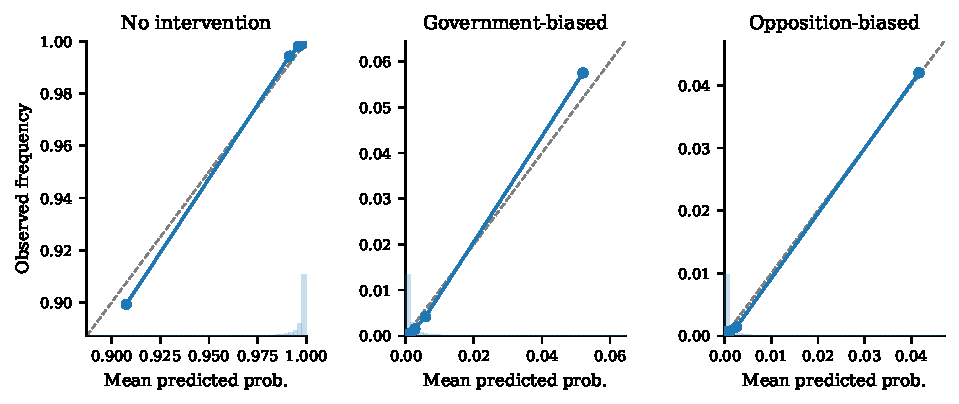
\includegraphics[width=\textwidth]{fig-sl-calibration.pdf}
  \caption{Reliability diagrams for each outcome class (no intervention,
    government-biased, opposition-biased).  Each panel plots observed
    frequency against mean predicted probability in 10 quantile bins,
    pooled across all 25 imputation draws; the dashed diagonal represents
    perfect calibration.  Axes are zoomed to the range where data reside.
    Shaded histograms show the distribution of predicted probabilities.}
  \label{fig:sl-calibration}
\end{figure}

\subsection{Fixed-Point Convergence}
\label{app:fp}

This appendix documents a Stage~1 \textit{training} diagnostic---whether the
spatial lags fed to the classifier are self-consistent with the probabilities
it predicts.  It is distinct from the universal Nash fixed point that constructs
the country-year shadow (Section~\ref{sec:constructing}), which operates over all
directed dyads rather than the training sample.

\subsubsection{The Consistency Requirement}

The spatial lags \texttt{spat\_gov} and \texttt{spat\_opp} enter the Stage~1 classifier as
predictors: they summarize how other potential interveners in the same conflict
are behaving, weighted by ideological similarity.  But the classifier itself
produces predicted intervention probabilities, and it is those probabilities---rather
than the realized 0/1/2 outcomes---that should, in principle,
enter the spatial weights.  The reason is that observed outcomes are single
draws from mixed-strategy equilibrium probabilities; a government-biased
intervention (outcome 1) carries no information about whether the intervening
state was playing a pure or mixed strategy.

Formally, the requirement is \textit{self-consistency}: the spatial lags fed into
$\hat{M}$ should be the weighted sums of the probabilities that $\hat{M}$ itself
assigns to each dyad.  Let $\hat{\mathbf{p}} = \hat{M}(\mathbf{X}(\mathbf{s}))$ be the
vector of predicted probabilities, where $\mathbf{X}(\mathbf{s})$ denotes the
feature matrix with spatial lags computed from $\mathbf{s}$.  Self-consistency
requires $\mathbf{s} = W \hat{\mathbf{p}}$, a fixed-point condition.

\subsubsection{Diagnosis of Non-Convergence}

The main training loop (Section~\ref{sec:constructing}) runs five rounds of
retrain-then-update, initializing $\mathbf{s}^{(0)}$ from the realized binary
outcomes.  Whether five rounds reach self-consistency is measured by the
residual at the five-iteration approximation $\mathbf{s}^{(5)}$: the mean
absolute gap between $\mathbf{s}^{(5)}$ and the weighted predictions
$W\hat{\mathbf{p}}(\mathbf{s}^{(5)})$ it should equal, which is exactly the
correction the first burnout pass applies:

\begin{equation*}
\Delta^{(5)} = \frac{1}{n} \sum_i \bigl| [W\hat{\mathbf{p}}(\mathbf{s}^{(5)})]_i - s_i^{(5)} \bigr|.
\end{equation*}

Averaged across all onset rows, both lag channels, and the 25 draws,
$\Delta^{(5)} \approx \BurnoutStart$---roughly \BurnoutStartX{} times the
$10^{-4}$ self-consistency threshold.  Five training rounds do not, on their
own, reach self-consistency.

\subsubsection{Frozen-Model Burnout}

Retraining the full super-learner is computationally expensive (${\sim}$3 hours per
draw).  An alternative is \textit{frozen-model burnout}: after training is complete,
hold the fitted $\hat{M}$ fixed and iterate spatial lags using its predictions
until convergence.  Each burnout pass costs only a prediction sweep
(milliseconds versus hours).

The burnout algorithm is:
\begin{enumerate}
\item Initialize from the five-iteration approximation $\mathbf{s}^{(5)}$.
\item Apply $\hat{M}$ to features $\mathbf{X}(\mathbf{s}^{(k)})$ to obtain $\hat{\mathbf{p}}^{(k)}$.
\item Update $\mathbf{s}^{(k+1)} = W \hat{\mathbf{p}}^{(k)}$.
\item If $\max_i |s_i^{(k+1)} - s_i^{(k)}| < \tau$, stop; otherwise go to step~2.
\end{enumerate}

The tolerance is set at $\tau = 5 \times 10^{-4}$.  This is above the
theoretical $10^{-4}$ threshold because random-forest predictions have
intrinsic stochasticity (different prediction calls can return slightly different
probabilities for the same input due to tree-averaging over bootstrap samples).
Empirical experiments confirm that $\Delta$ plateaus around $5 \times 10^{-4}$ and
cannot be reduced further without retraining.

Across all 25 imputation draws, burnout converges in \BurnoutLo--\BurnoutHi{} iterations (mean
\BurnoutMean), with final $\Delta$ ranging from $\BurnoutDeltaLo \times 10^{-4}$ to
$\BurnoutDeltaHi \times 10^{-4}$---confirming that the plateau reflects irreducible
prediction noise rather than failure to converge.  Figure~\ref{fig:fp-convergence} shows the
convergence trajectories: all draws exhibit rapid geometric decay (roughly
halving each iteration) before plateauing at the tolerance threshold.

\begin{figure}[t]
  \centering
  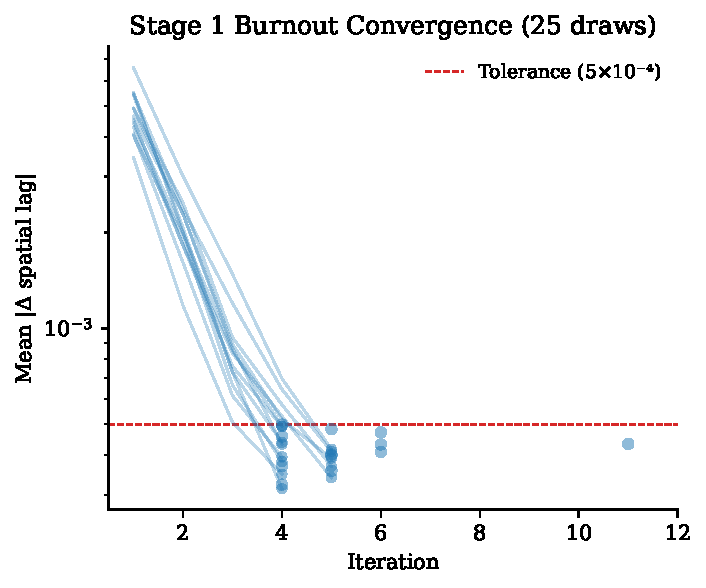
\includegraphics[width=0.85\textwidth]{fig-fp-convergence.pdf}
  \caption{Burnout convergence across all 25 imputation draws.  Each line traces
  the per-iteration mean $|\Delta\text{spatial lag}|$ from the five-iteration
  approximation to convergence; dots mark endpoints.  Dashed line: convergence
  tolerance ($5 \times 10^{-4}$).}
  \label{fig:fp-convergence}
\end{figure}

\subsubsection{Interpretation: Approximate Equilibrium Selection}

The burnout iteration does not find an equilibrium of the underlying
intervention game; it finds a fixed point of the \textit{fitted classifier} $\hat{M}$.
The procedure is a nonparametric instance of the nested pseudo-likelihood
(NPL) algorithm of \citet{aguirregabiriamira2007}: where
A\&M iterate between estimating structural parameters and updating choice
probabilities, the present application holds the fitted $\hat{M}$ fixed and
iterates only the spatial lags (choice probabilities), corresponding to
A\&M's two-step PML with a nonparametric first stage.
These coincide with the true equilibrium only if $\hat{M}$ exactly recovers the
true equilibrium mapping, which no finite-sample estimator can guarantee.

The weaker, defensible claim is as follows.  Realized outcomes are draws from
\textit{some} equilibrium of the underlying game---they satisfy Nash consistency by
assumption, since they were generated by the players.  But the equilibrium
correspondence for a game of this scale (up to \MaxInterveners{} potential interveners, each
choosing a mixed strategy) generically admits multiple equilibria, and different
conflict cases may be near different connected components.  The realized binary
outcomes provide only coarse information about which equilibrium each case is
near: a 0/1/2 outcome is consistent with any mixed strategy that places positive
probability on that action.

The burnout iteration uses the model to extract additional information.  Given
the realized action as a starting condition, iterating the model refines the
estimated spatial lags toward values that are approximately consistent with the
smooth probability distribution implied by $\hat{M}$.  In this sense, the
iteration performs \textit{approximate equilibrium selection}: it identifies, for each
conflict case, which region of the equilibrium correspondence the realized
outcome is most consistent with, according to the model's learned mapping.

Three caveats are important.  First, the model is trained on spatial lags
derived from realized outcomes (the five-iteration warm start), not from the
burnout-converged values.  Retraining on the converged values would raise a
circularity concern: the model's weights would depend on predictions the model
itself generated.  By freezing the model before burnout, the learned coefficients
remain anchored to the training-time feature distribution, and the converged
lags represent a small perturbation ($\Delta \approx 0.003$ relative to the warm
start) rather than a wholesale shift to a foreign equilibrium.  Second, the
equilibrium selected for each training case by the burnout need not be the same
equilibrium that governs prediction-time cases.  The identifying assumption is
that the equilibrium selection mechanism is stable across the sample---the same
forces that push cases toward particular equilibria in training also govern
unobserved cases.  Third, the burnout-converged lags are used only to compute
the shadow measure (the country-year expectations $E_\text{gov}$ and $E_\text{opp}$ in
Stage~2) and not to re-estimate Stage~1.  The shadow measure therefore reflects
the approximately-equilibrium spatial environment, while the classifier's
weights remain from training on the realized-outcome initialization.

\section{Properties of the Shadow Measure}
\label{app:properties}

This appendix documents the descriptive behavior of $E^G$ and $E^O$,
summarized in Section~\ref{sec:shadow-properties} of the main text.

Before turning to the onset analysis, I examine the descriptive properties
of $E^G$ and $E^O$ to establish that they behave as the theory predicts.

The dyad-level predictions reveal a structural asymmetry between the two
sides of intervention.  The highest predicted probabilities of
government-biased intervention involve superpowers projecting influence into
client states---the United States supporting the Philippines in 1972
($\hat{p}_\text{gov} = \pGovMax$), Laos in 1962, and Cambodia in 1971.  For
opposition-biased intervention, the picture shifts: the maximum is Israel
opposing the Syrian government in 1982 ($\hat{p}_\text{opp} = \pOppMax$), followed
by Bulgaria targeting Greece in 1946 and Kuwait targeting Iraq in 1991,
and nine of the ten highest-ranked opposition predictions involve non-P5
interveners.  A measurement framework restricted to P5 states
would miss the majority of the opposition-biased shadow.

Table~\ref{tab:shadow-dyads} makes this concrete for three canonical onsets, reporting
the five states to which the classifier assigns the highest government- and
opposition-biased intervention probabilities alongside an indicator of whether
the state actually intervened in that direction.

% AUTO-GENERATED by scripts/export_numbers.py -- DO NOT EDIT.
\begin{table}[t]
  \centering
  \small
  \setlength{\tabcolsep}{4pt}
  \begin{tabular}{@{}lr c @{\quad} lr c@{}}
    \toprule
    \textbf{Gov-biased} & $\hat{p}$ & & \textbf{Opp-biased} & $\hat{p}$ & \\
    \midrule
    \multicolumn{6}{c}{\textbf{Angola (1976) --- 5 actual interventions}} \\
    \cmidrule(lr){1-6}
    United States$^\ast$ & .26 &  & Zaire & .49 &  \\
    Cuba & .15 & $\checkmark$ & South Africa & .21 & $\checkmark$ \\
    USSR$^\ast$ & .15 & $\checkmark$ & United States$^\ast$ & .04 & $\checkmark$ \\
    Congo & .07 &  & Congo & .04 &  \\
    Zambia & .07 &  & Portugal & .04 &  \\
    \addlinespace
    \multicolumn{6}{c}{\textbf{Ethiopia (1978) --- 4 actual interventions}} \\
    \cmidrule(lr){1-6}
    USSR$^\ast$ & .17 & $\checkmark$ & Somalia & .39 & $\checkmark$ \\
    Cuba & .16 & $\checkmark$ & United States$^\ast$ & .07 &  \\
    United States$^\ast$ & .14 &  & North Yemen & .06 &  \\
    Kenya & .05 &  & Sudan & .04 &  \\
    China$^\ast$ & .04 &  & Cuba & .02 &  \\
    \addlinespace
    \multicolumn{6}{c}{\textbf{Afghanistan (1978) --- 4 actual interventions}} \\
    \cmidrule(lr){1-6}
    USSR$^\ast$ & .15 & $\checkmark$ & Pakistan & .20 & $\checkmark$ \\
    China$^\ast$ & .09 &  & China$^\ast$ & .08 &  \\
    United Kingdom$^\ast$ & .09 &  & Iran & .07 & $\checkmark$ \\
    Iran & .09 &  & United States$^\ast$ & .03 & $\checkmark$ \\
    United States$^\ast$ & .05 &  & United Kingdom$^\ast$ & .02 &  \\
    \bottomrule
  \end{tabular}
  \caption{Top five predicted interveners for three canonical onsets; out-of-fold
    probabilities averaged across the 25 imputation draws.  $^\ast$P5 member;
    $\checkmark$ the state actually intervened in that direction (Regan coding).}
  \label{tab:shadow-dyads}
\end{table}


Across the three cases, \DyadHits{} actual interventions appear in the top five
on the correct side---and in each case, restricting the measure to P5 states
would discard the single most important opposition-biased intervener: Zaire
in Angola, Somalia in Ethiopia, Pakistan in Afghanistan.\footnote{%
  The United States appears in the top five government-biased predictions for
  all three cases, yet actually intervened on the opposition side in Angola and
  Afghanistan.  The model assigns substantial probability mass to \textit{both} sides
  but defaults toward government-biased intervention because that is the modal
  US posture across the full sample.  This directional ambiguity for superpowers
  is one reason the country-year aggregation is preferable to raw dyad-level
  predictions: summing across all potential interveners preserves the correct
  signal that these countries faced unusually high total intervention pressure,
  even where the classifier hedges on which side a specific superpower would take.}

Figure~\ref{fig:shadow-kde} shows the cross-sectional distribution of $E^G$ and $E^O$
across all country-years.  Both measures are heavily right-skewed: the
median country-year faces modest intervention expectations, but a long
right tail captures the handful of states embedded in dense alliance
networks and superpower competition.

\begin{figure}[t]
  \centering
  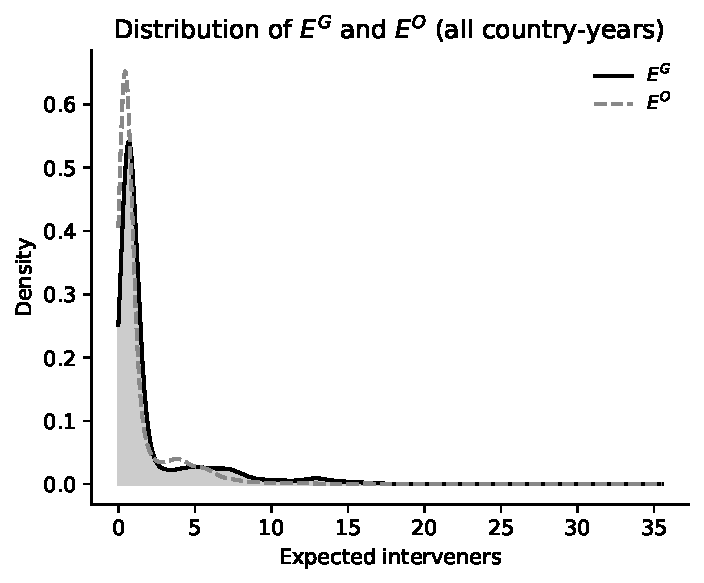
\includegraphics[width=0.85\textwidth]{fig-shadow-kde.pdf}
  \caption{Kernel density estimates of $E^G$ and $E^O$ across all
    country-years (1946--2014), averaged across 25 imputation draws.}
  \label{fig:shadow-kde}
\end{figure}

Figure~\ref{fig:shadow-ts} traces the temporal dynamics for three of the most
heavily internationalized civil wars of the Cold War.  Beyond magnitude, the
shadow recovers \textit{direction}---which outside powers line up on which
side.  Angola is the clearest case: at the 1976 onset the government-side
shadow ($E^G = \ShAngolaG$) is anchored by Cuba and the Soviet Union, the
MPLA's patrons, while the opposition-side shadow ($E^O = \ShAngolaO$) loads on
Zaire, South Africa, and the United States---the external backers of the FNLA
and UNITA.  Ethiopia shows the same structure through the 1978 realignment:
Cuba and the Soviet Union again anchor the government side for the Derg
($E^G = \ShEthiopiaG$), while Somalia drives the opposition side in the Ogaden war.  Afghanistan illustrates a regime switch: the 1978 Saur Revolution
lifts the government-side shadow, but by 1979 the opposition side overtakes it
($E^O = \ShAfghanO$ vs.\ $E^G = \ShAfghanG$), capturing the surge of mujahideen
support from Pakistan, Iran, and the United States against a Soviet-backed
government.  In every case the shadow concentrates on the historically correct
interveners rather than diffusing across the system---evidence that it tracks
the strategic environment, not merely the onsets on which Stage~1 is trained.

\begin{figure}[t]
  \centering
  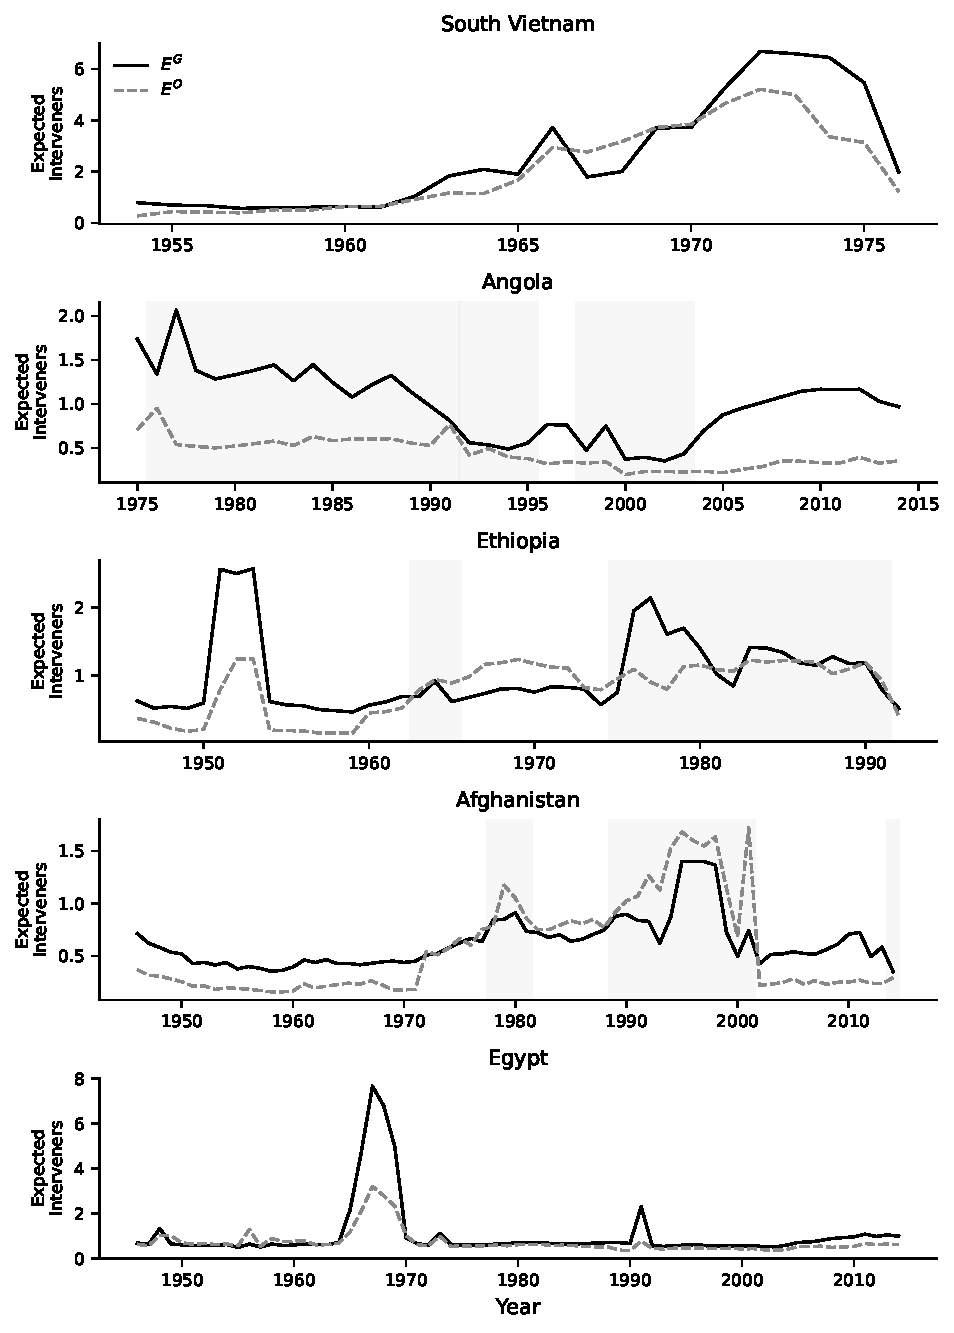
\includegraphics[width=0.85\textwidth]{fig-shadow-ts.pdf}
  \caption{Shadow measure time series ($E^G$ and $E^O$) for three countries
    with well-documented intervention environments.  Probabilities averaged
    across 25 imputation draws.}
  \label{fig:shadow-ts}
\end{figure}

$E^G$ correlates positively with both existing measures of anticipated
intervention: the Lake security hierarchy used by \citet{cunningham2016}
($r = \CorrLake$, $n = \NLake$) and the structural P5 intervention probabilities
estimated by \citet{gibilisco2022} ($r = \CorrGM$, $n = \NGM$).  The stronger
correlation with G\&M is expected---both capture intervention propensity
directly---while the moderate hierarchy correlation reflects the fact that
US dominance is only one component of the broader intervention environment.

\section{Full Second-Stage Estimates}
\label{app:full-model}

Table~\ref{tab:direction-full} reports the complete \textit{Entrants} onset
model whose two shadow coefficients are summarized, in the identified
net-tilt parameterization, in Table~\ref{tab:direction}.  Coefficients and
intervals are computed by the $T \times P$ procedure, so the intervals
propagate the shadow's measurement uncertainty and are correspondingly wide
for the collinear shadow channels; the controls are conventionally estimated.

% AUTO-GENERATED by scripts/export_numbers.py -- DO NOT EDIT.
\begin{table}[t]
  \centering
  \begin{tabular}{@{}lrr@{}}
    \toprule
    & Coef. & 95\% $T\times P$ interval \\
    \midrule
    $\gamma^G$ (gov.-biased shadow) & $-1.61$ & $[-6.14,\ +0.43]$ \\
    $\gamma^O$ (opp.-biased shadow) & $+0.19$ & $[-2.53,\ +1.97]$ \\
    \midrule
    Constant & $-12.01$ & $[-38.25,\ +14.28]$ \\
    Democracy & $-0.03$ & $[-0.06,\ -0.00]$ \\
    Log GDP per capita & $-0.44$ & $[-0.79,\ -0.11]$ \\
    Log population & $+0.12$ & $[-0.08,\ +0.31]$ \\
    Mountainous terrain & $+0.13$ & $[-0.09,\ +0.31]$ \\
    Noncontiguous & $+0.51$ & $[-0.18,\ +1.12]$ \\
    Oil exporter & $+0.25$ & $[-0.27,\ +0.79]$ \\
    New state & $+1.20$ & $[+0.22,\ +2.00]$ \\
    Political instability & $+0.71$ & $[+0.29,\ +1.22]$ \\
    Prior war & $+0.75$ & $[+0.15,\ +1.39]$ \\
    Ethnic frac. & $+0.50$ & $[-0.28,\ +1.37]$ \\
    Religious frac. & $+0.93$ & $[-0.21,\ +2.07]$ \\
    Year trend & $+0.00$ & $[-0.01,\ +0.02]$ \\
    \bottomrule
  \end{tabular}
  \caption{The full \textit{Entrants} onset model.  Coefficients are $T \times P$
    means; intervals are the 2.5th--97.5th percentiles.  Net tilt
    $= (\gamma^O - \gamma^G)/2$, common intensity $= (\gamma^O + \gamma^G)/2$.}
  \label{tab:direction-full}
\end{table}


% Source: scripts/mh_chisq.py, scripts/spike_rf_significance.py, scripts/rfsig_perdraw.py;
% results/spike/mh_chisq_{calib,focal,40pt,joint_seeds}.parquet, rfsig_summary.parquet,
% rfsig_perdraw.parquet (seeded, committed).
\section{Predictive-Significance Tests}
\label{app:pstests}

Table~\ref{tab:dropcol} scores each covariate by what its removal costs a
held-out forecast.  This section reports the formal counterpart: the
prediction-difference test of \citet{mentchhooker2016}, the procedure
\citet{mcalexandermentch2020} bring to onset data.  Trees are built on
subsamples ($k = 75$ of $n = \OosN$; minimum split 3), so ensemble
predictions are asymptotically normal U-statistics with estimable covariance;
the test compares an ensemble built on the observed data against one built
with the focal columns permuted, evaluating both at $N$ held-out test points
and referring $\hat{D}' \hat{\Sigma}_D^{-1} \hat{D}$ to $\chi^2_N$.
Following the original authors' discipline, the tuning was validated on
calibration anchors before any shadow test was run: across \MhNoiseReps\
pure-noise focal columns the $p$-values are near-uniform (mean
$\MhNoiseMean$; $\MhNoiseHits$ at or below $0.05$, the nominal rate), and a
synthetic strong signal is rejected decisively
($\chi^2_{20} = \MhSynthStat$).

Verdicts at any single set of test points are variable in a rare-event
outcome---the original authors note the test's sensitivity to test-point
location---so the joint test of the two shadow channels, the appropriate
test for a collinear pair, was run across ten independent test-point draws
(five each at $N = 20$ and $N = 40$) and combined by twice the median
$p$-value \citep{meinshausen2009}.  It rejects at every configuration:
\MhJointTight\ draws at $p \le 0.005$, all ten at $p \le \MhJointMaxP$,
combined $p \approx \MhJointComb$ at both test-set sizes.  The marginal
tests are configuration-sensitive in exactly the way collinearity
predicts---each channel's verdict depends on which test points happen to
separate it from its twin---the same pathology \citet{mcalexandermentch2020}
document for the fractionalization measures in the Fearon--Laitin model, and
the empirical motivation for working in the tilt and intensity combinations
of Section~\ref{sec:direction}.  The structural controls do not reject
(income $p = \MhGdpP$, population $p = \MhPopP$).

A conventional permutation counterpart agrees: refit the ensemble under each
of $99$ draws from the focal columns' permutation null, score each refit out
of fold, and compare the observed average precision to that null---the
brute-force analogue of the computationally efficient test of
\citet{coleman2022}.  This version permits the generated-regressor honesty
the asymptotic machinery does not contemplate: run separately on each of the
\PdDraws\ measurement draws, the joint test rejects at $p \le 0.05$ in
\PdJointDraws\ (median $\PdJointMed$, worst $\PdJointMax$), and the marginals
clear conventional thresholds in most draws ($E^G$ in \PdEgovHits\ of
\PdDraws, $E^O$ in \PdEoppHits) while remaining draw-sensitive.  The
measurement spread does not rescue the null.


\end{document}
